\PassOptionsToPackage{pdfpagelabels=false}{hyperref} 
\documentclass{entcs} 
\usepackage{entcsmacro}
\usepackage{graphicx}
\usepackage{pgfplots}
\usepackage{amsmath}
%\setlength{\paperheight}{11in}
\usepackage[noend]{algpseudocode}
\usepackage{fancyvrb}
\usepackage{subfigure}
\pgfplotsset{
    compat=1.15,
    %every axis legend/.append style={at={(0.5,-0.13)},anchor=north,legend cell align=left},
    legend pos=north west,
    legend style={draw=none,
              text width=0.9in,           %% adjust
              %minimum height=0.5in,     %% adjust
              %anchor=center,
              %cells={anchor=west},
            },
    %axis lines=left,
}
\sloppy
\newcommand{\acm}[3]{\{#1\}\rightarrow#3}
\newcommand{\ac}[3]{$\{#1\}\rightarrow#3$}
\newcommand{\omesi}{^\omega_\alpha}
% Macros relatives à la traduction de PH avec arcs neutralisants vers PH à k-priorités fixes

% Macros générales
%\newcommand{\ie}{\textit{i.e.} }
\newcommand{\segm}[2]{\llbracket #1; #2 \rrbracket}
%\newcommand{\f}[1]{\mathsf{#1}}

% Notations générales pour PH
\newcommand{\PH}{\mathcal{PH}}
%\newcommand{\PHs}{\mathcal{S}}
\newcommand{\PHs}{\Sigma}
%\newcommand{\PHp}{\mathcal{P}}
\newcommand{\PHp}{\textcolor{red}{\mathcal{P}}}
%\newcommand{\PHproc}{\mathcal{P}}
\newcommand{\PHproc}{\mathbf{Proc}}
\newcommand{\Proc}{\PHproc}
\newcommand{\PHh}{\mathcal{H}}
\newcommand{\PHa}{\PHh}
%\newcommand{\PHa}{\mathcal{A}}
\newcommand{\PHl}{\mathcal{L}}
\newcommand{\PHn}{\mathcal{N}}

\newcommand{\PHhitter}{\mathsf{hitter}}
\newcommand{\PHtarget}{\mathsf{target}}
\newcommand{\PHbounce}{\mathsf{bounce}}
%\newcommand{\PHsort}{\Sigma}
\newcommand{\PHsort}{\PHs}

%\newcommand{\PHfrappeur}{\mathsf{frappeur}}
%\newcommand{\PHcible}{\mathsf{cible}}
%\newcommand{\PHbond}{\mathsf{bond}}
%\newcommand{\PHsorte}{\mathsf{sorte}}
%\newcommand{\PHbloquant}{\mathsf{bloquante}}
%\newcommand{\PHbloque}{\mathsf{bloquee}}

%\newcommand{\PHfrappeR}{\textcolor{red}{\rightarrow}}
%\newcommand{\PHmonte}{\textcolor{red}{\Rsh}}

\newcommand{\PHhitA}{\rightarrow}
\newcommand{\PHhitB}{\Rsh}
%\newcommand{\PHfrappe}[3]{\mbox{$#1\PHhitA#2\PHhitB#3$}}
%\newcommand{\PHfrappebond}[2]{\mbox{$#1\PHhitB#2$}}
\newcommand{\PHhit}[3]{#1\PHhitA#2\PHhitB#3}
\newcommand{\PHfrappe}{\PHhit}
\newcommand{\PHhbounce}[2]{#1\PHhitB#2}
\newcommand{\PHobj}[2]{\mbox{$#1\PHhitB^*\!#2$}}
\newcommand{\PHobjectif}{\PHobj}
\newcommand{\PHconcat}{::}
%\newcommand{\PHneutralise}{\rtimes}
\def\Sce{\mathbf{Sce}}

% Actions plurielles
\newcommand{\PHhitmultsymbol}{\rightarrowtail}
\newcommand{\PHhitmult}[2]{\mbox{$#1 \PHhitmultsymbol #2$}}
\newcommand{\PHfrappemult}{\PHhitmult}
\newcommand{\PHfrappemults}[2]{\PHhitmult{\{#1\}}{\{#2\}}}

\def\PHget#1#2{{#1[#2]}}
%\newcommand{\PHchange}[2]{#1\langle #2 \rangle}
%\newcommand{\PHchange}[2]{(#1 \Lleftarrow #2)}
%\newcommand{\PHarcn}[2]{\mbox{$#1\PHneutralise#2$}}
\newcommand{\PHplay}{\cdot}

\newcommand{\PHstate}[1]{\mbox{$\langle #1 \rangle$}}
\newcommand{\PHetat}{\PHstate}

\def\supp{\mathsf{support}}
\def\first{\mathsf{first}}
\def\last{\mathsf{last}}

\def\DNtrans{\rightarrow_{ADN}}
\def\DNdef{(\mathbb F, \langle f^1, \dots, f^n\rangle)}
\def\DNdep{\mathsf{dep}}
\def\PHPtrans{\rightarrow_{PH}}
\def\get#1#2{#1[{#2}]}
\def\encodeF#1{\mathbf{#1}}
\def\toPH{\encodeF{PH}}
\def\card#1{|#1|}
\def\decode#1{\llbracket#1\rrbracket}
\def\encode#1{\llparenthesis#1\rrparenthesis}
\def\Hits{\PHa}
\def\hit{\PHhit}
\def\play{\cdot}

\def\Pint{\textsc{PINT}}



\usepackage{ifthen}

\newcommand{\currentScope}{}
\newcommand{\currentSort}{}
\newcommand{\currentSortLabel}{}
\newcommand{\currentAlign}{}
\newcommand{\currentSize}{}

\newcounter{la}
\newcommand{\TSetSortLabel}[2]{
  \expandafter\repcommand\expandafter{\csname TUserSort@#1\endcsname}{#2}
}
\newcommand{\TSort}[4]{
  \renewcommand{\currentScope}{#1}
  \renewcommand{\currentSort}{#2}
  \renewcommand{\currentSize}{#3}
  \renewcommand{\currentAlign}{#4}
  \ifcsname TUserSort@\currentSort\endcsname
    \renewcommand{\currentSortLabel}{\csname TUserSort@\currentSort\endcsname}
  \else
    \renewcommand{\currentSortLabel}{\currentSort}
  \fi
  \begin{scope}[shift={\currentScope}]
  \ifthenelse{\equal{\currentAlign}{l}}{
    \filldraw[process box] (-0.5,-0.5) rectangle (0.5,\currentSize-0.5);
    \node[sort] at (-0.2,\currentSize-0.4) {\currentSortLabel};
   }{\ifthenelse{\equal{\currentAlign}{r}}{
     \filldraw[process box] (-0.5,-0.5) rectangle (0.5,\currentSize-0.5);
     \node[sort] at (0.2,\currentSize-0.4) {\currentSortLabel};
   }{
    \filldraw[process box] (-0.5,-0.5) rectangle (\currentSize-0.5,0.5);
    \ifthenelse{\equal{\currentAlign}{t}}{
      \node[sort,anchor=east] at (-0.3,0.2) {\currentSortLabel};
    }{
      \node[sort] at (-0.6,-0.2) {\currentSortLabel};
    }
   }}
  \setcounter{la}{\currentSize}
  \addtocounter{la}{-1}
  \foreach \i in {0,...,\value{la}} {
    \TProc{\i}
  }
  \end{scope}
}

\newcommand{\TTickProc}[2]{ % pos, label
  \ifthenelse{\equal{\currentAlign}{l}}{
    \draw[tick] (-0.6,#1) -- (-0.4,#1);
    \node[tick label, anchor=east] at (-0.55,#1) {#2};
   }{\ifthenelse{\equal{\currentAlign}{r}}{
    \draw[tick] (0.6,#1) -- (0.4,#1);
    \node[tick label, anchor=west] at (0.55,#1) {#2};
   }{
    \ifthenelse{\equal{\currentAlign}{t}}{
      \draw[tick] (#1,0.6) -- (#1,0.4);
      \node[tick label, anchor=south] at (#1,0.55) {#2};
    }{
      \draw[tick] (#1,-0.6) -- (#1,-0.4);
      \node[tick label, anchor=north] at (#1,-0.55) {#2};
    }
   }}
}
\newcommand{\TSetTick}[3]{
  \expandafter\repcommand\expandafter{\csname TUserTick@#1_#2\endcsname}{#3}
}

\newcommand{\myProc}[3]{
  \ifcsname TUserTick@\currentSort_#1\endcsname
    \TTickProc{#1}{\csname TUserTick@\currentSort_#1\endcsname}
  \else
    \TTickProc{#1}{#1}
  \fi
  \ifthenelse{\equal{\currentAlign}{l}\or\equal{\currentAlign}{r}}{
    \node[#2] (\currentSort_#1) at (0,#1) {#3};
  }{
    \node[#2] (\currentSort_#1) at (#1,0) {#3};
  }
}
\newcommand{\TSetProcStyle}[2]{
  \expandafter\repcommand\expandafter{\csname TUserProcStyle@#1\endcsname}{#2}
}
\newcommand{\TProc}[1]{
  \ifcsname TUserProcStyle@\currentSort_#1\endcsname
    \myProc{#1}{\csname TUserProcStyle@\currentSort_#1\endcsname}{}
  \else
    \myProc{#1}{process}{}
  \fi
}

\newcommand{\repcommand}[2]{
  \providecommand{#1}{#2}
  \renewcommand{#1}{#2}
}
\newcommand{\THit}[5]{
  \path[hit] (#1) edge[#2] (#3#4);
  \expandafter\repcommand\expandafter{\csname TBounce@#3@#5\endcsname}{#4}
}
\newcommand{\TBounce}[4]{
  (#1\csname TBounce@#1@#3\endcsname) edge[#2] (#3#4)
}

%\newcommand{\TState}[1]{
%  \foreach \proc in {#1} {
%    \node[current process] (\proc) at (\proc.center) {};
%  }
%}

\newcommand{\TState}[1]{
  \foreach \proc in {#1} {
        \node[current process] (\proc) at (\proc.center) {};
  };
}
\newcommand{\TCoopHit}[6]{
  \node[#2, apdot] at (#3) {};
  \foreach \proc in {#1} {
    \draw[#2,-] (#3) edge (\proc);
  }
  \path[hit] (#3) edge[#2] (#4#5);
  \expandafter\repcommand\expandafter{\csname TBounce@#4@#6\endcsname}{#5}
}

% ex : \TAction{c_1}{a_1.west}{a_0.north west}{}{right}
% #1 = frappeur
% #2 = cible
% #3 = bond
% #4 = style frappe
% #5 = style bond
\newcommand{\TAction}[5]{
  \THit{#1}{#4}{#2}{}{#3}
  \path[bounce, bend #5=50] \TBounce{#2}{}{#3}{};
}

% ex : \TActionPlur{f_1, c_0}{a_0.west}{a_1.south west}{}{3.5,2.5}{left}
% #1 = frappeur
% #2 = cible
% #3 = bond
% #4 = style frappe
% #5 = coordonnées point central
% #6 = direction bond
\newcommand{\TActionPlur}[6]{
  \TCoopHit{#1}{#4}{#5}{#2}{}{#3}
  \path[bounce, bend #6=50] \TBounce{#2}{}{#3}{};
}

% procedure, abstractions and dependencies
\newcommand{\abstr}[1]{#1^\wedge}%\text{\textasciicircum}}
\def\BS{\mathbf{BSeq}}
\def\aBS{\abstr{\BS}}
\def\abeta{\abstr{\beta}}
\def\aZ{\abstr{\zeta}}
\def\aY{\abstr{\xi}}

\def\beforeproc{\vartriangleleft}

\def\powerset{\wp}

\def\Sce{\mathbf{Sce}}
\def\OS{\mathbf{OSeq}}
\def\Obj{\mathbf{Obj}}
%\def\Proc{\mathbf{Proc}}
%\def\Sol{\mathbf{Sol}}
\newcommand{\Sol}{\mathbf{Sol}}
\newcommand{\NSol}{\Sol}
\newcommand{\sSol}{\mathbf{Sync}}

\usepackage{galois}
\newcommand{\theOSabstr}{toOS}
\newcommand{\OSabstr}[1]{\theOSabstr(#1)}
\newcommand{\theOSconcr}{toSce}
\newcommand{\OSconcr}[1]{\theOSconcr(#1)}

% \def\gO{\mathbb{O}}
% \def\gS{\mathbb{S}}
\def\aS{\mathcal{A}}
\def\Req{\mathrm{Req}}
%\def\Sol{\mathrm{Sol}}
\def\Cont{\mathrm{Cont}}
\def\cBS{\BS_\ctx}
\def\caBS{\aBS_\ctx}
\def\caS{\aS_\ctx}
\def\cSol{\Sol_\ctx}
\def\cReq{\Req_\ctx}
\def\cCont{\Cont_\ctx}

\def\any{\star}

% \def\gProc{\mathrm{maxPROC}}
\def\mCtx{\mathrm{maxCtx}}

%\def\procs{\f{procs}}
\def\objs{\f{objs}}
\def\sat#1{\lceil #1\rceil}

\def\gCont{\f{maxCont}}
\def\lCont{\f{minCont}}
\def\lProc{\f{minProc}}
\def\gProc{\f{maxProc}}

\def\join{\oplus}
\def\concat{\!::\!}
\def\emptyseq{\varepsilon}
\def\ltw{\preccurlyeq_{\OS}}
\def\indexes#1{\mathbb{I}^{#1}}
%\def\indexes#1{\{1..|#1|\}}
\def\supp{\f{support}}
\def\w{\omega}
\def\W{\Omega}
% \def\ctx{\varsigma}
%\def\ctx{{\textcolor{green}{s}}}
% \def\ctx{s}
% \def\Ctx{\mathbf{Ctx}}
\def\Ctx{\mathbf{Ctx}}
\def\mconcr{\gamma}
\def\concr{\mconcr_s}
\def\obj#1#2{{#1\!\Rsh^*\!\!#2}}
\def\objp#1#2#3{\obj{{#1}_{#2}}{{#1}_{#3}}}
\def\A{\mathcal{A}}
\def\cwA{\A_\ctx^\w}
\def\cwReq{\Req_\ctx^\w}
\def\cwSol{\Sol_\ctx^\w}
\def\cwCont{\Cont_\ctx^\w}
\def\gCtx{\f{maxCtx}}
\def\endCtx{\f{endCtx}}
\def\ceil{\f{end}}

%\def\lfp{\mathrm{lfp}\;}
%\def\mlfp#1{\mathrm{lfp}\{#1\}\;}
\newcommand{\lfp}[3]{\mathbf{lfp}\{#1\}\left(#2\mapsto#3\right)}
\def\maxobjs{{\f{maxobjs}}}
\def\maxprocs{{\f{maxprocs}_\ctx}}
\def\objends{{\f{ends}}}

\def\ra{\rho}
\def\rb{\rho^\wedge}
\def\rc{\widetilde{\rho}}
\def\interleave{\f{interleave}}

\def\join{\concat}

\tikzstyle{aS}=[every edge/.style={draw,->,>=stealth}]
\tikzstyle{Asol}=[draw,circle,minimum size=5pt,inner sep=0,node distance=1cm]
\tikzstyle{Aproc}=[draw,node distance=1cm]
\tikzstyle{Aobj}=[node distance=1.5cm]
\tikzstyle{Anos}=[font=\Large]
\tikzstyle{Assol}=[node distance=1.2cm]
%\tikzstyle{AprocPrio}=[Aproc,double]
\tikzstyle{AsolPrio}=[Asol,double]
\tikzstyle{AprocPrio}=[Aproc,double]
\tikzstyle{aSPrio}=[aS,double]


\newcommand{\startl}[1]{\node[Aproc] (#1) {$#1$};\node[Asol,right of=#1] (#1s) {};\path (#1) edge (#1s);}%start link
\newcommand{\link}[2]{\node[Aproc,right of=#1s] (#2) {$#2$};\node[Asol,right of=#2] (#2s) {};\path (#1s) edge (#2) (#2) edge (#2s);} %normal link
\newcommand{\specl}[3]{\node[Aproc,#1 right of=#2s] (#3) {$#3$};\node[Asol,right of=#3] (#3s) {};\path (#2s) edge (#3) (#3) edge (#3s);} %special link
\newcommand{\edl}[2]{\node[Assol,right of=#1s] (#1st){$\varnothing$};\path (#1s) edge (#1st);}%end link


%\def\procs{\mathsf{procs}}
%\def\allprocs{\mathsf{allProcs}}
%\def\allprocs{\procs}
%\def\pfp{\mathsf{pfp}}
\def\pfp{\mathsf{focals}^1}
\def\pfpprocs{\mathsf{pfpProcs}}
\def\bounceprocs{\mathsf{bounceProcs}}
\def\newprocs{\mathsf{newProcs}}

\def\aB{\mathcal{B}}
\def\sat#1{{#1}}
%\def\sat#1{\lceil #1\rceil}
\newcommand{\thisB}[2]{\sat{\aB_{#2}^{#1}}}
\newcommand{\myp}{u}
%\def\cwB{\thisB{\myp}{\ctx}}
\def\cwB{\thisB{\myp}{s}}
%\def\cwB{\sat{\aB_\ctx^\w}}
%\def\cwBz{\thisB{\myp}{\ctx_0}}
\def\cwBz{\thisB{\myp}{s_0}}
\def\mycwB#1#2{\sat{\aB_{#1}^{#2}}}
\def\Bsol{\sat{\Sol^\w_\ctx}}
\def\Breq{\sat{\Req^\w_\ctx}}
\def\Bcont{\sat{\Cont^\w_\ctx}}

\def\myB{\aB^\myp_\ctx}
\def\mysol{\overline{\Sol^\w_\ctx}}
\def\myreq{\overline{\Req^\w_\ctx}}
\def\mycont{\overline{\Cont^\w_\ctx}}

\newcommand{\csState}{\mathsf{procState}}

\newcommand{\V}{V}
\newcommand{\E}{E}
\newcommand{\cwV}{\V_s^\myp}
\newcommand{\cwE}{\E_s^\myp}
% \newcommand{\cwV}{\V_\ctx^\myp}
% \newcommand{\cwE}{\E_\ctx^\myp}
%\newcommand{\VProc}{\textcolor{red}{\V_\PHproc}}
%\newcommand{\VObj}{\textcolor{red}{\V_\Obj}}
%\newcommand{\VSol}{\V_{Sol}}
%\newcommand{\VSol}{\textcolor{red}{\V_{\Sol}}}
\newcommand{\VProc}{\V \cap \PHproc}
\newcommand{\VObj}{\V \cap \Obj}
\newcommand{\VSol}{\V \cap \Sol}
\newcommand{\cwVProc}{\cwV \cap \PHproc}
\newcommand{\cwVObj}{\cwV \cap \Obj}
\newcommand{\cwVSol}{\cwV \cap \Sol}
\newcommand{\cwVsSol}{\cwV \cap \sSol}

\def\Bv{\sat{\cwV}}
\def\Be{\sat{\cwE}}
\def\BvProc{\textcolor{red}{\sat{\cwV}^\PHproc}}
\def\BvObj{\textcolor{red}{\sat{\cwV}^\Obj}}
%\def\BvSol{\sat{\cwV}^{Sol}}
\def\BvSol{\textcolor{red}{\sat{\cwV}^{\Sol}}}

\def\cwBNodes{\Bv}
\def\cwBEdges{\Be}
\def\nsol{\f{nsol}}
\def\conn{\f{conn}}

\newcommand{\Bee}[2]{\Be^{#1}_{#2}}

%\def\mlfp#1{\f{pppf}\{#1\}}

\def\PHobjp#1#2#3{\PHobj{{#1}_{#2}}{{#1}_{#3}}}
\def\Obj{\mathbf{Obj}}
\def\powerset{\wp}
\def\gCont{\f{maxCont}}

\def\muconcr{\ell}
\def\uconcr{\muconcr_\ctx}

% Styles TikZ et couleurs personnalisées

\usepackage{tikz}

\newdimen\pgfex
\newdimen\pgfem
\usetikzlibrary{arrows,shapes,shadows,scopes}
\usetikzlibrary{positioning}
\usetikzlibrary{matrix}
\usetikzlibrary{decorations.text}
\usetikzlibrary{decorations.pathmorphing}
\usetikzlibrary{arrows,shapes}

\definecolor{lightgray}{rgb}{0.8,0.8,0.8}
\definecolor{lightgrey}{rgb}{0.8,0.8,0.8}

\definecolor{lightred}{rgb}{1,0.8,0.8}
\definecolor{lightgreen}{rgb}{0.7,1,0.7}
\definecolor{darkgreen}{rgb}{0,0.5,0}
\definecolor{darkblue}{rgb}{0,0,0.5}
\definecolor{darkyellow}{rgb}{0.5,0.5,0}
\definecolor{lightyellow}{rgb}{1,1,0.6}
\definecolor{darkcyan}{rgb}{0,0.6,0.6}
\definecolor{lightcyan}{rgb}{0.6,1,1}
\definecolor{darkorange}{rgb}{0.8,0.2,0}
\definecolor{notsodarkred}{rgb}{0.8,0,0}

\definecolor{notsodarkgreen}{rgb}{0,0.7,0}

%\definecolor{coloract}{rgb}{0,1,0}
%\definecolor{colorinh}{rgb}{1,0,0}
\colorlet{coloract}{darkgreen}
\colorlet{colorinh}{red}
\colorlet{coloractgray}{lightgreen}
\colorlet{colorinhgray}{lightred}
\colorlet{colorinf}{darkgray}
\colorlet{coloractgray}{lightgreen}
\colorlet{colorinhgray}{lightred}

\colorlet{colorgray}{lightgray}
\colorlet{colorhl}{blue}


\tikzstyle{boxed ph}=[]
\tikzstyle{sort}=[fill=lightgray, rounded corners, draw=black]
\tikzstyle{process}=[circle,draw,minimum size=15pt,fill=white,font=\footnotesize,inner sep=1pt]
%\tikzstyle{black process}=[process, draw=blue, fill=red,text=black,font=\bfseries]
\tikzstyle{gray process}=[process, draw=black, fill=lightgray]
\tikzstyle{highlighted process}=[current process, fill=gray]
\tikzstyle{process box}=[fill=none,draw=black,rounded corners]
\tikzstyle{current process}=[process, draw=black, fill=lightgray]
%\tikzstyle{current process}=[process,fill=lightcyan]
\tikzstyle{hl process}=[process,fill=blue!30]
\tikzstyle{tick label}=[font=\footnotesize]
\tikzstyle{tick}=[densely dotted] %-
\tikzstyle{hit}=[->,>=angle 45]
\tikzstyle{selfhit}=[min distance=50pt,curve to]
\tikzstyle{bounce}=[densely dotted,>=stealth',->]
\tikzstyle{ulhit}=[draw=lightgray,fill=lightgray]
\tikzstyle{pulhit}=[fill=lightgray]
\tikzstyle{bulhit}=[draw=lightgray]
\tikzstyle{hl}=[very thick,colorhl]
\tikzstyle{hlb}=[very thick]
\tikzstyle{hlhit}=[hl]
%\tikzstyle{hl2}=[hl]
%\tikzstyle{nohl}=[font=\normalfont,thin]

\tikzstyle{update}=[draw,->,dashed,shorten >=.7cm,shorten <=.7cm]

\tikzstyle{unprio}=[draw,thin]%[double]
%\tikzstyle{prio}=[draw,thick,-stealth]%[double]
\tikzstyle{prio}=[draw,-stealth,double]

\tikzstyle{hitless graph}=[every edge/.style={draw=red,-}]

\tikzstyle{aS}=[every edge/.style={draw,->,>=stealth}]
\tikzstyle{Asol}=[draw,circle,minimum size=5pt,inner sep=0,node distance=1cm]
\tikzstyle{Aproc}=[draw,node distance=1.2cm]
\tikzstyle{Aobj}=[node distance=1.5cm]
\tikzstyle{Anos}=[font=\Large]

\tikzstyle{AsolPrio}=[Asol,double]
\tikzstyle{AprocPrio}=[Aproc,double]
\tikzstyle{aSPrio}=[aS,double]

\colorlet{colorhlwarn}{notsodarkred}
\colorlet{colorhlwarnbg}{lightred}
\tikzstyle{Ahl}=[very thick,fill=colorhlwarnbg,draw=colorhlwarn,text=colorhlwarn]
\tikzstyle{Ahledge}=[very thick,double=colorhlwarnbg,draw=colorhlwarn,color=colorhlwarn]





%\definecolor{darkred}{rgb}{0.5,0,0}



\tikzstyle{grn}=[every node/.style={circle,draw=black,outer sep=2pt,minimum
                size=15pt,text=black}, node distance=1.5cm, ->]
\tikzstyle{inh}=[>=|,-|,draw=colorinh,thick, text=black,label]
\tikzstyle{act}=[->,>=triangle 60,draw=coloract,thick,color=coloract]
\tikzstyle{inhgray}=[>=|,-|,draw=colorinhgray,thick, text=black,label]
\tikzstyle{actgray}=[->,>=triangle 60,draw=coloractgray,thick,color=coloractgray]
\tikzstyle{inf}=[->,draw=colorinf,thick,color=colorinf]
%\tikzstyle{elabel}=[fill=none, above=-1pt, sloped,text=black, minimum size=10pt, outer sep=0, font=\scriptsize,draw=none]
\tikzstyle{elabel}=[fill=none,text=black, above=-2pt,%sloped,
minimum size=10pt, outer sep=0, font=\scriptsize, draw=none]
%\tikzstyle{elabel}=[]


\tikzstyle{plot}=[every path/.style={-}]
\tikzstyle{axe}=[black,->,>=stealth']
\tikzstyle{ticks}=[font=\scriptsize,every node/.style={black}]
\tikzstyle{mean}=[thick]
\tikzstyle{interval}=[line width=5pt,red,draw opacity=0.7]
%\definecolor{lightred}{rgb}{1,0.3,0.3}

%\tikzstyle{hl}=[yellow]
%\tikzstyle{hl2}=[orange]

%\tikzstyle{every matrix}=[ampersand replacement=\&]
%\tikzstyle{shorthandoff}=[]
%\tikzstyle{shorthandon}=[]
\tikzstyle{objective}=[process,very thick,fill=yellow!50]

\tikzstyle{coopupdate}=[-stealth,decorate,decoration={zigzag,amplitude=1.5pt,post=lineto,post length=.3cm,pre=lineto,pre length=.3cm}]

\tikzstyle{labelprio}=[circle, fill=blue!30, inner sep=0pt, minimum size=13pt]
\tikzstyle{labelprio1}=[labelprio]
\tikzstyle{labelprio2}=[labelprio, fill=red!60]
\tikzstyle{labelprio3}=[labelprio, fill=orange!50]
\tikzstyle{labelprio4}=[labelprio, fill=brown!50]

\tikzstyle{labelstocha}=[rectangle, rounded corners=4pt]

\tikzstyle{andot}=[circle, fill=black, inner sep=1.2pt, draw=transparent]
\tikzstyle{anligne}=[thick]

\tikzstyle{apdot}=[andot] %[circle, fill=black, draw=black, inner sep=1]
\tikzstyle{apdotsimple}=[] %[circle, fill=black, draw=black, inner sep=1]

% Figure de résumé des liens entre les formalismes
\tikzstyle{equiv-externe}=[thick, rounded corners, draw=gray, fill=gray!10, align=center,
  inner sep=8]

% label pour les délais des actions 
 \tikzstyle{labeldelai1}=[circle, fill=red!60, inner sep=0pt, minimum size=8pt]
  \tikzstyle{labeldelai2}=[circle, fill=blue!30, inner sep=0pt, minimum size=8pt]
  \tikzstyle{labeldelai3}=[circle, fill=brown!50, inner sep=0pt, minimum size=8pt]
  \tikzstyle{labeldelai4}=[circle, fill=green!50, inner sep=0pt, minimum size=8pt]
  
% Automata Networks:
\tikzstyle{local transitions}=[->,>=latex',thick,bend left=30,
               every node/.style={fill=white,inner sep=1pt,outer sep=1pt}]
\tikzstyle{reach}=[fill=lightgray,ellipse]

\tikzstyle{local transitions 2}=[->,>=latex',thick,bend left=100,
               every node/.style={fill=white,inner sep=1pt,outer sep=4pt}]

\tikzstyle{local transitions 3}=[->,>=latex',thick,bend right=100,
               every node/.style={ right, fill=white,inner sep=1pt,outer sep=4pt}]
               
% Graphe d'états
% noeuds
\tikzstyle{vide}= [rectangle, minimum width=2em,minimum height=1.5em,]
\tikzstyle{stable}= [rectangle,fill=lightred]
\tikzstyle{current}= [rectangle,fill=lightcyan]
\tikzstyle{initial}= [rectangle,fill=green!20]

% % STG transitions
\tikzstyle{etiquette}=[midway,fill=blue!20,circle,scale=0.7pt]
\tikzstyle{etiquette2}=[midway,fill=green!20,circle,scale=0.7pt]
%
\tikzstyle{currentTrans}=[->,very thick,blue]
\tikzstyle{seperatedTransPart1}=[draw, thick, blue]
\tikzstyle{seperatedTransPart2}=[->, thick, blue]


\tikzstyle{mytext}=[thick, text width=4.5em,inner sep=1pt]
\tikzstyle{line} =[draw, thick, -latex',shorten >=2pt]
\tikzstyle{block} =[rectangle,text width=6em,draw,minimum height=4em, outer sep=0pt]

\tikzstyle{adn}=[every node/.style={circle,draw=black,outer sep=2pt,minimum
                size=15pt,text=black}, node distance=1.5cm, ->]
                
% Définition des nouvelles options xmin, xmax, ymin, ymax
% Valeurs par défaut : -3, 3, -3, 3
\tikzset{
    xmin/.store in=\xmin, xmin/.default=-3, xmin=-3,
    xmax/.store in=\xmax, xmax/.default=3, xmax=3,
    ymin/.store in=\ymin, ymin/.default=-3, ymin=-3,
    ymax/.store in=\ymax, ymax/.default=3, ymax=3,
}
% Commande qui trace la grille entre (xmin,ymin) et (xmax,ymax)
\newcommand {\grille}
    {\draw[help lines] (\xmin,\ymin) grid (\xmax,\ymax);}
% Commande \axes
\newcommand {\axes} {
    \draw[->] (\xmin,0) -- (\xmax+0.5,0);
    \draw[->] (0,\ymin) -- (0,\ymax+0.5);
}
% Commande qui limite l’affichage à (xmin,ymin) et (xmax,ymax)
\newcommand {\fenetre}
    {\clip (\xmin,\ymin) rectangle (\xmax,\ymax);}
   
 \newcommand{\nombresCopiesParNote}
   {(0,0)(1,0)(2,2)(3,0)(4,6)(5,4)(6,7)(7,4)(8,3)(9,0)(10,1)}  
% Expression level of a
 \newcommand{\expressionDiscreteA}
   {(0,0)(1,0)(2,0)(3,0)(4,0)(4,1)(5,1)(5,0)(6,0)(7,0)(8,0)(9,0)(9,1)(10,1)(11,1)(12,1)(13,1)(13,0)(14,0)(15,0)(16,0)(17,0)(17,1)(18,1)}      
   
% Expression level of b
 \newcommand{\expressionDiscreteB}
   {(0,1)(12,1)(12,0)(18,0)} 
   
% Expression level of z
 \newcommand{\expressionDiscreteZ}
   {(0,0)(3,0)(3,1)(14,1)(14,0)(18,0)}
\def\lastname{Chai, Ribeiro, Magnin, Roux, Inoue}
\begin{document}
\begin{frontmatter}
    \title{Static Analysis and Stochastic Search for Reachability Problem} 
    \author{Xinwei Chai, Tony Ribeiro, Morgan Magnin, Olivier Roux\thanksref{ALL}\thanksref{myemail}}
    \address{Laboratoire des Sciences du Num\'erique de Nantes
            \\ 1 Rue de la No\"e, 44300 Nantes, France}
    \author{Katsumi Inoue\thanksref{coemail}}
    \address{National Institute of Informatics\\ 
            2-1-2 Hitotsubashi, Chiyoda-ku, Tokyo 101-8430, Japan} 
    \thanks[ALL]{Supported by China Scholarship Council} 
    \thanks[myemail]{Email: \href{mailto:myuserid@mydept.myinst.myedu} {\texttt{\normalshape \{xinwei.chai, tony.ribeiro, morgan.magnin, olivier.roux\}@ls2n.fr}}}
    \thanks[coemail]{Email: \href{mailto:couserid@codept.coinst.coedu} {\texttt{\normalshape
        inoue@nii.ac.jp}}}
\begin{abstract} 
This paper focuses on a major improvement on the analysis of reachability properties in large-scale dynamical biological models. 
To tackle such models, where classical model checkers fail due to state space explosion led by  exhaustive search.
Alternative static analysis approaches have been proposed, but they may also fail in certain cases due to non-exhaustive search.
In this paper, we introduce a hybrid approach ASPReach, which combines static analysis and stochastic search to break the limits of both approaches.
We tackle this issue on a modeling framework we recently introduced, Asynchronous Binary Automata Network (ABAN). 
We show that ASPReach is able to analyze efficiently some reachability properties which could not be solved by existing methods.
We studied also various cases from biological literature, emphasizing the merits of our approach in terms of conclusiveness and performance.
\end{abstract}
\begin{keyword}
Model checking, Reachability problem, Asynchronous Binary Automata Network, Local Causality Graph, Heuristics, Answer Set Programming.
\end{keyword}
\end{frontmatter}
\section{Introduction}\label{intro}
With increasing quantities of available data provided by new technologies, \textit{e.g.} DNA microarray \cite{marx2013}, there is a growing need for expressive modelings and their related high-performance analytic tools. 
Among them, works on concurrent systems have been of interest in systems biology for over a decade \cite{bockmayr2002using,bortolussi2008modeling,wiley2003computational}. 
If model validation is a major concern, one of the main challenges nowadays is predicting the behavior of these systems. 

Reachability problem on formal models is a critical challenge where both validation problems (whether the model satisfies the \textit{a priori} knowledge) and prediction problems (properties to be discovered) meet. 
From a formal point of view, numerous biological properties in computational models can be transformed to reachability properties. 
For example, the reachability of state 0/1 of a could represent the activation/inhibition of certain gene or synthesis of a protein, while initial state could represent initial observation in an experiment.
If the reachability of a certain state contradicts with the \textit{a priori} knowledge, one can modify the model and/or design a new experiment to verify whether there is an error in the \textit{a priori} knowledge or former observation. 
Also, reachability analysis is of help to medicine design: for example if one wants to prevent the carcinogenesis of a cell (target state), one possible solution is to find the critical pathways towards the target state and design a medicine to cut them in order to keep the cell healthy.

%State of the art
In the domain of model checking, reachability has been of great interest for over 30 years \cite{clarke2008birth,clarke20142}. 
Various modeling frameworks and semantics in bioinformatics have been studied: Boolean network \cite{akutsu2007control}, Petri nets \cite{mayr1984,esparza1998}, timed-automata \cite{Daws1998,wozna2003}. 
These approaches rely on global search and thus face state explosion problem as the state space grows exponentially with the number of variables. 
In \cite{peterson1977petri}, it has been shown that the reachability problem of Petri net is exponential time-hard and exponential space-hard, and this conclusion does not change even under some specific conditions \cite{esparza1998}. 
For 1-safe Petri nets, the complexity of reachability analysis is generally PSPACE-complete \cite{cheng1995complexity}.
Li \textit{et al.} \cite{li2012reachability,li2014stability} investigated theoretically the stability, the controllability and the reachability of Switched Boolean Networks, but their method remains computationally expensive;
Saadatpour \textit{et al.} \cite{saadatpour2010attractor} researched only the reachability of fixed points.

To tackle the complexity issue, symbolic model checking \cite{burch1992symbolic} based on ordered binary decision diagrams (OBDDs) and SAT-solvers (satisfiability) \cite{abdulla2000symbolic} have been studied over years, but still fail to analyze big biological systems with more than $1000$ variables. 
Bounded Model Checking (BMC) \cite{clarke2001bounded} is an efficient approach but generally not complete as its searching depth is limited to a given integer $k$.

Beside these approaches, abstraction is an efficient strategy to deal with such models of big scale. 
It aims at approximating the model while keeping the most important parts influencing the reachability.
Abstract methods often have better time-memory performance but with a loss of information. 
They solve usually a simplified version of the original model, i.e. the results from these approaches are not necessarily compatible with all the properties of the original model.
While studying reachability problems, the system dynamics is abstracted to static causalities between states and transitions.

%Related work
We have designed a new discrete modeling framework for a concurrent system \cite{chai2018heuristic}: Asynchronous Binary Automata Network (ABAN).
In ABAN, we applied the approach developed by Paulev\'e \textit{et al.} \cite{pauleve2017reduction,folschette2015,pauleve2011} to address reachability problem.
This approach refers to a static abstraction of the reachability (with an over-approximation and an under-approximation of the real dynamics).
It is based on an abstract interpretation: Local Causality Graph (LCG). 
This interpretation drastically reduces the searching state-space thus avoids costly global search \cite{pauleve2012}. 
However, this pure static analysis is not complete as there are inconclusive cases which can not be decided reachable or not.

Many biological networks are encoded in Boolean style, \textit{e.g.} \cite{akutsu2007control,kauffman1969}, because BN is a simple formalism but with strong applicability: discretization in BN is a way to handle the imprecision of \textit{a priori} knowledge on the model.
However BN may be not expressive enough.
As to the modeling of the dynamic behavior ``$a\gets$ $1$ at moment $t+1$ if $b=1$ at moment $t$'', one has $a(t+1)=b(t)$ in BN.
$a$ always follows the evolution of $b$ but with a potentially unwanted behavior ``$a\gets 0$ when $b=0$ at moment $t$''.
ABAN models this dynamics as \textit{via} \ac{b_1}{a_0}{a_1} without this redundancy. 
Besides, BNs are transformable to ABANs, and this property makes our approach applicable to a wider domain (Appendix \ref{appendix:trans}).

%Contribution
Our work shares similar concerns but we combine static analysis and bounded model checking.
We have developed a heuristic approach PermReach to attack reachability problem \cite{chai2018heuristic} which is more conclusive than pure static analysis but time-consuming and still not able to solve reachability problems under certain conditions.
In this paper, we propose a hybrid approach ASPReach based on the former LCG reasoning and a non-exhaustive search in the LCG to obtain a more conclusive solution of reachability problems.
%Novelty
ASPReach allows one to solve the cases where other static methods fail.
Furthermore, it can also solve the reachability of a set of states which to our knowledge has never been done in static way.
We assess the value of our contribution using benchmarks on biological examples from the literature.%Answer Set Programming(ASP) is an efficient tool for solving difficult search problems, many of them are NP-hard.

This paper is organized as follows: Section 2 introduces the formal background and the formalization necessary to the understanding of the work; Section 3 presents the concrete methods and algorithms composing the whole approach; Section 4 shows the benchmarks evaluating our approach and other alternatives; Section 5 concludes this paper.

\section{Formalization}
\textit{Notations}:

$a_i$ means automaton $a$ is taking value $i$;

$x::y$ is the sequential connector of entities $x$ and $y$, where $x$ appears just before $y$;

$a.next$ is the immediate successor of $a$; $a.pred$ is the immediate predecessor of $a$.

Boolean Network is a traditional and efficient modeling framework, with many biological networks encoded in BN \cite{kauffman1969}.
To describe the dynamical properties more precisely, Automata Network is introduced \cite{chai2018heuristic,plateau1991stochastic}. 
It can be considered as a subset of communicating finite state machines or safe Petri Nets.

Asynchronous Binary Automata Network (ABAN) is a special case of Automata Network.  
``Asynchronous'' implies the update scheme that no more than one automaton can change its value at a time.
Asynchronous update scheme makes a trade-off between the biological reality and complexity.
From a given state, biological systems may evolve to multiple future states (e.g. cell differentiation), but it is costly to simulate generalized ANs where arbitrary subsets of automata can be updated simultaneously.
``Binary'' implies that every automaton has exactly two possible states $(0,1)$.  In Appendix \ref{appendix:trans}, we show how to transform a Boolean Network into ABAN.

\begin{definition}[ABAN]
    An ABAN is a triplet $AB = (\Sigma,L,T)$, where:
    \begin{itemize}
    \item $\Sigma\triangleq\{a,b,\ldots\}$ is the finite set of automata with every component having a Boolean state;
    \item $LS\triangleq \underset{a\in \Sigma}{\cup} \{a_0,a_1\}$ is the set of all local states, $L\triangleq \underset{a\in \Sigma'}{\times} \{a_0,a_1\}$ is the set of joint states where $\Sigma'\subseteq\Sigma$. Particularly, if $\Sigma'=\Sigma$, $L$ is the set of global states. 
    \item $T\triangleq \{A\rightarrow b_i\mid b\in \Sigma \land A\in L\}$ is the set of transitions, where $A$ (called head) is the set of required state(s) for transition $tr=A\to b_i$ , which allows to flip $b_{1-i}$ to $b_i$ (called body). In other words, transition $tr$ is said fireable iff $A\subseteq s$, where $s$ is the current global state.
    \end{itemize}
\end{definition}

A local state represents the state of \textit{one} automaton, e.g. $a_1$, while a global state represents the \textit{joint state} of all the automata in the network, e.g. $\langle a_0, b_1,c_0 \rangle$ where $L=\{a,b,c\}$. 

\begin{definition}[Asynchronous Dynamics]
    From current global state $s$, the global state after firing transition $tr=A\to b_i$ is denoted $s \cdot tr = s \setminus \{b_{1-i}\} \cup \{b_i\}$, where $b_{1-i} \in s$.
    The state of a certain automaton $a$ is noted $(s\cdot tr)[a]$.
    Particularly, if there is no fireable transition, the next state remains the same as the current state.
\end{definition}

To describe the evolution in an ABAN, we use the notion of trajectory.
\begin{definition}[Trajectory]
Given an ABAN $AB = (\Sigma,L,T)$ and a global initial state $\alpha\in L$, a trajectory $t$ from $\alpha$ is a sequence of transitions $t=tr_1::\cdots :: tr_i::\cdots ::tr_n$ with $tr_i\in T$ and each $tr_i$ is fireable in $(s \cdot tr_1 \cdot \ldots \cdot tr_{i-1})$.
From $\alpha$, the global state after firing all transitions of $t$ is $(s \cdot tr_1 \cdot \ldots \cdot tr_n)$, denoted $s \cdot t$.
\end{definition}

\begin{definition}[State sequence]
Given an ABAN $AB = (\Sigma,L,T)$ and a global initial state $\alpha\in L$ and trajectory $t$, the state sequence $seq=s_1::\cdots :: s_i::\cdots ::s_n$ with $s_i\in LS$ is formed by the updated local states during the trajectory $t$.
\end{definition}


\begin{example}
    Fig. \ref{exampleABAN} shows an ABAN with initial state $\alpha=\langle a_0,b_0,c_0,d_0,e_0\rangle$ and a possible trajectory is $t=\acm{d_0}{b_0}{b_1}::\acm{b_1}{d_0}{d_1}::\acm{d_1}{c_0}{c_1}::\acm{b_1,c_1}{a_0}{a_1}$.
    After firing the transitions in trajectory $t$, the state becomes $\Omega=s\cdot t=\langle a_1,b_1,c_1,d_1,e_0\rangle$, and $\omega= a_1= (\alpha\cdot t)[a]$. The state sequence is $seq=b_1::d_1::c_1::a_1$.
\end{example}

\begin{figure}[ht]
\centering
\begin{tikzpicture}[apdotsimple/.style={apdot},scale=0.7, every node/.style={scale=0.8}]
\scriptsize
\TSort{(0,0)}{a}{2}{l}
\TSort{(2,0)}{b}{2}{l}
\TSort{(4,0)}{c}{2}{l}
\TSort{(6,0)}{d}{2}{l}
\TSort{(8,0)}{e}{2}{l}

% with delays
\path[local transitions]

	(a_0) edge node[auto] {\{$b_1, c_1$\}} (a_1)
    (a_0) edge[bend right] node[right] {$\{e_1\}$} (a_1)
	(b_0) edge node[auto] {$\{d_0\}$} (b_1)
	(d_0) edge node[auto] {$\{b_1\}$} (d_1)
	%(c_1) edge node[auto] {$\{b_0\}$, $2$} (c_0)
	(c_0) edge node[auto] {$\{d_1\}$} (c_1)
;

\TState{a_0, b_0, c_0, d_0,e_0}


\end{tikzpicture}

\caption{An example of ABAN}\label{exampleABAN}
\end{figure}
As to reachability problem, given an ABAN $AB= (\Sigma,L,T)$, the joint reachability $REACH (\Omega)$ is formalized as: joint state $\Omega$ is reachable iff there exists a trajectory $t$ s.t. $\alpha\cdot t=\Omega$.
Partial reachability $reach(\omega)$ is defined analogously: local state $\omega=a_i$ is reachable iff there exists a trajectory $t$ s.t. $(\alpha\cdot t)[a]=a_i$.
$REACH (\Omega)$ and $reach(\omega)$ take Boolean values \textbf{True}, \textbf{False} or \textbf{Inconclusive} if it cannot be decided.
In Fig. \ref{exampleABAN}, $\Omega=\langle a_1,b_1,c_1,d_1,e_0\rangle$ or $\omega=a_1$ is reachable from initial state $\alpha$ \textit{via} trajectory $t$, \textit{i.e.} $reach(a_1)=\textbf{True}$ and $REACH(\Omega)=\textbf{True}$. 
In fact, the reachability of a joint state even a global state is equivalent to that of one local state. 
Given a set of target states $\{a_i,\ldots z_j\}$, by adding a new automaton $x$ to $\Sigma$, setting its initial state to $x_0$ and adding transition $\acm{a_i,\ldots z_j}{x_0}{x_1}$ to $T$, $REACH(\{a_i,\ldots z_j\})$ is thus equivalent to $reach(x_1)$. For convenience, we study partial reachabilities in this paper.

Paulev\'e \textit{et al.} \cite{pauleve2011} have proposed Local Causality Graph (LCG) to analyze reachability problems statically.
LCG abstracts the original problem through an over-approximation (necessary condition) and an under-approximation (sufficient condition).
It is a very efficient tool as there is no global search and all the operations are bounded in polynomial complexity.
However LCG does not guarantee to obtain a result, i.e. some inconclusive instances satisfy the necessary condition and fail sufficient conditions.
In this paper, we make use of LCG by removing some elements needed only in multivalued networks, then we try to analyze it more deeply to solve inconclusive cases of binary valued systems.
In fact, Didier \textit{et al.} have shown a technique to transform a multivalued network to Boolean network \cite{didier2011mapping}, which provides us the applicability to multivalued situations.
\begin{definition}[LCG]\label{defLCG}
Given an ABAN $AB = (\Sigma,L,T)$, an initial state $\alpha$ and a target state $\omega$, LCG $l= (V_{\mathrm{state}},V_{\mathrm{solution}},E)$ is the smallest recursive structure with $E \subseteq (V_{\mathrm{state}}\times V_{\mathrm{solution}})\cap (V_{\mathrm{solution}}\times V_{\mathrm{state}})$ which satisfies:
\begin{eqnarray*}
    \omega&\in& V_{\mathrm{state}} \\
    a_i\in V_{\mathrm{state}} &\Leftrightarrow& \{ (a_i, sol_{a_i})| a_i\in \alpha\}\subseteq E \\
    sol_{a_i}\in V_{\mathrm{solution}}&\Leftrightarrow& \{ (sol_{a_i},\mathbf{V}_a (sol_{a_i})\}\subseteq E
\end{eqnarray*}
where $V_{\mathrm{state}}\subseteq LS$ is the set of local states, $V_{\mathrm{solution}}\subseteq T$ is the set of solutions and $\mathbf{V}_a$ is the set of required local states of $sol_{a_i}$.
\end{definition}
\begin{example}
    Fig. \ref{LCGexample} shows the LCG for analyzing $reach(a_1)$ in Fig. \ref{exampleABAN}.
    \begin{figure}[ht]
        \centering
        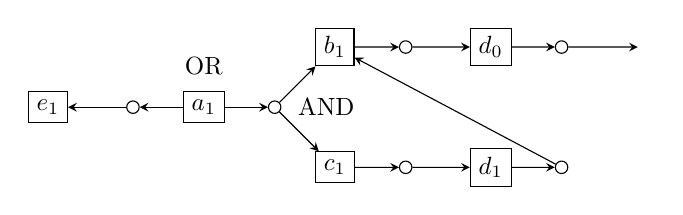
\begin{tikzpicture}[aS,scale=0.9, every node/.style={scale=0.9}]  
  	
  	\startl{a_1};
    \node[Asol,left of=a_1] (a_1s1){};
    \node[Aproc,left of=a_1s1] (e_1){$e_1$};
    \node[right = 0.1cm of a_1s] {AND};
    \node[above = 0.1cm of a_1] {OR};
    \path 
    (a_1s1) edge (e_1)
    (a_1) edge (a_1s1)
    ; 
  	\specl{above}{a_1}{b_1};
  	\link{b_1}{d_0};
  	\edl{d_0};
  	\specl{below}{a_1}{c_1};
	\link{c_1}{d_1};
    \path (d_1s) edge (b_1);
\end{tikzpicture}

        \caption{Visualization of LCG, with the squares representing local states and small circles representing solution nodes.
        $\varnothing$ signifies that there is no need to link any transitions, i.e the former state $d_0$ is in the initial state.}
        \label{LCGexample}
    \end{figure}
\end{example}

Algorithm \ref{AlgConstructLCG} describes how to construct an LCG from an ABAN $AB = (\Sigma,L,T)$.
Starting from  a given target state $Ls=\omega$, one can find all the transitions $T_s\subseteq T$ reaching $\omega$ and add edges $\omega \to T_s$.
Then we find all the heads $A$ of $T_s$ and add edges $T_s \to A$ and replace $Ls$ with $A$ (recursion).
Finally, we update the structure until $Ls\subseteq \alpha$ or there is no transition with body in $Ls$.

\begin{algorithm}[htb]
\begin{algorithmic}
\State Input: an ABAN $AB=(\Sigma,L,T)$, an initial state $\alpha$, a target state $\omega$
\State Output: LCG $l=(V_{\mathrm{state}},V_{\mathrm{solution}}, E)$
\State Initialization: 
$Ls\gets \{\omega\}$, $V_{\mathrm{state}}\gets\varnothing$, $V_{\mathrm{solution}}\gets \varnothing$, $E\gets \varnothing$
\While{$Ls\neq \varnothing$}
    \State $Ls=Ls\backslash V_{\mathrm{state}}$
	\For{$a_i\in Ls$}
		\State $Ls\gets Ls\backslash \{a_i\}$
		\If{$a_i\in \alpha$}
			%\State $a_i{\rm .next}=sol_{a_i}$
			%\State $V_{\mathrm{solution}}\gets V_{\mathrm{solution}}\cup \{(a_i,\varnothing)\} $
			\State $E\gets E\cup \{(a_i,\varnothing)\} $
            %\State $sol_{a_i}{\rm .next}=\varnothing$
    	\Else
    	    \State{\textcolor{gray}{// Choose the transitions reaching $a_i$, i.e. with body $a_{1- i}$}}
    		\For{$sol=A\to a_{1- i}\in T$}
    		    \State $V_{\mathrm{solution}}\gets V_{\mathrm{solution}}\cup \{sol\}$
    		    \State $E\gets E\cup \{(a_i,sol)\} $
    			%\State $a_i{\rm .next}\gets a_i{\rm .next}\cup sol$
    			\State $V_{\mathrm{state}}\gets V_{\mathrm{state}}\cup {A}$
    			\For{$b_j\in A$}
    				%\State $sol{\rm .next}\gets b_j$
    				\State $E\gets E\cup \{(sol,b_j)\} $
    			\EndFor
    			\State $Ls\gets Ls\cup A$
                \State $V_{\mathrm{state}}\gets V_{\mathrm{state}}\cup Ls$
    		\EndFor
    		\State$V_{\mathrm{solution}}\gets V_{\mathrm{solution}}\cup a_i{\rm .next}$           
    	\EndIf
	\EndFor
\EndWhile
\State\Return{$(V_{\mathrm{state}},V_{\mathrm{solution}},E)$}
\end{algorithmic}
\caption{Construction of LCG}\label{AlgConstructLCG}
\end{algorithm}

When the recursive construction finishes, LCG is in fact a digraph with vertices $V$ consisting of $V_{\mathrm{state}}$ and $V_{\mathrm{solution}}$. 
$E$ is a set of the edges between state nodes and solution nodes. 
To access certain local state $a_i$, at least one of the transitions of the form $X\to a_i$ has to be fireable, i.e. $a_i$ needs to have at least one successor solution node, thus state nodes are \textbf{OR gates}; similarly, to make one transition (solution node) fireable, all of its successor state nodes need to be reached simultaneously, i.e. solution nodes are \textbf{AND gates}. 
A recursive reasoning of reachability begins with a state node representing desired target state, go through $a_i\mapsto sol_{a_i}\mapsto b_j \cdots$ and ends with initial state (reachable) or a local state with no solution successor (unreachable).

With LCG, it is easy to verify whether their are potential pathways from the target state $\omega$ to the initial state $\alpha$.
If there does not exist such a pathway, one can ensure that $\omega$ is not reachable from $\alpha$.
\cite{pauleve2012} explains this local reasoning.

\begin{definition}[Pseudo-reachability]\label{defPseudoReach}
Given an LCG $l=(V_{\mathrm{state}},V_{\mathrm{solution}},E)$ with global initial state $\alpha$, the pseudo-reachability of node $v\in V_{\mathrm{state}}$ is defined as
\begin{equation}
\nonumber
    reach'(\alpha,v)=
    \begin{cases}
        \mathrm{\bf True} & {\rm if\ } v\in \alpha\\
        \mathrm{\bf False} & {\rm if\ } v\not\in \alpha\ {\rm and} \not\exists(s,sol) \in E\\
        %\bigvee_{(s,sol) \in E} \mathrm{firable}(sol) & otherwise
        \bigvee_{(s,sol) \in E}  (\bigwedge_{(sol,s)\in E} reach'(\alpha,s)) & {\rm otherwise}
    \end{cases}
\end{equation}
%where $\mathrm{firable}(sol)=\bigwedge_{(sol,s)\in E} reach'(\alpha,s)$. 

\end{definition}

However, pseudo-reachability is named ``pseudo'' because it is only an over-approximation of reachability, i.e. it reveals a necessary condition of reachability.
\begin{example}
    In Fig. \ref{fig:limitation}, $reach'(l,c_1)=reach'(l,a_1)\land reach'(l,b_1)=reach'(l,a_0)\land reach'(l,b_0)=\textbf{True}$. Both $a_1$ and $b_1$ are reachable, but they can not be reached simultaneously.
    In such LCG, there are two branches, $a_1\mapsto b_0$ and $b_1\mapsto a_0$, the automata $a$ and $b$ involve themselves in different branches, the reachability of $a_1$ impedes the reachability of $b_1$ and \textit{vice versa}.
\end{example}

\begin{figure}[ht]
    \centering
    \begin{minipage}{0.4\textwidth}
\centering
\begin{tikzpicture}[apdotsimple/.style={apdot},scale=0.7, every node/.style={scale=0.8}]
\scriptsize
\TSort{(0,0)}{a}{2}{l}
\TSort{(2,0)}{b}{2}{l}
\TSort{(4.5,0)}{c}{2}{l}

% with delays
\path[local transitions]

	(c_0) edge node[auto] {\{$a_1, b_1$\}} (c_1)
	(a_0) edge node[auto] {\{$b_0$\}} (a_1)
	(b_0) edge node[auto] {\{$a_0$\}} (b_1)
;
\TState{a_0, b_0, c_0}
\end{tikzpicture}
\end{minipage}\hfill
\begin{minipage}{0.6\textwidth}
\centering
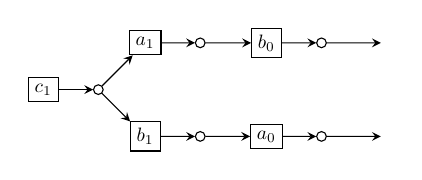
\begin{tikzpicture}[aS,scale=0.7, every node/.style={scale=0.7}]  
  	
  	\startl{c_1};
  	\specl{above}{c_1}{a_1};
  	\link{a_1}{b_0};
  	\edl{b_0};
  	\specl{below}{c_1}{b_1};
	\link{b_1}{a_0};
  	\edl{a_0};
\end{tikzpicture}
\end{minipage}
    \caption{$\Sigma=\{a,b,c\}$, $T=\{\acm{b_0}{a_0}{a_1},\ \acm{a_0}{b_0}{b_1},\ \acm{a_1,b_1}{c_0}{c_1}\},\omega=c_1$}
    \label{fig:limitation}
\end{figure}

Also, the recursive reasoning does not terminate if there exists cycles in LCG. 
While computing the pseudo-reachability, self-dependent form $reach'(l,a_i)=\ldots=reach'(l,a_i)$ will appear. 
Dealing with cycles becomes inevitable.

%Details will be discussed in Algorithm \ref{algOverall}.

\begin{definition}[Cycle]
In an LCG, a cycle is formed by a sequence of nodes linked as follows: $a_i\to \circ \to \cdots \to \circ \to a_i$
\end{definition}

To identify cycles, we search instead Strongly Connected Components (SCC) of size greater than one.
Because cycles may interlace and there is no such problem in SCC.
In other words, a SCC may contain several nested cycles which connect to each other.
\cite{tarjan1972} shows that the detection of SCCs can be done in $O (|V|+|E|)$ time, with $|V|$ the cardinality of the vertices and $|E|$ the cardinality of the edges.
LCG is usually a sparse graph, as in biological systems, the components mostly interact with only a part of the system, hence the out-degree can be considered of $O (1)$ and the detection of SCCs\footnote{Python3 implementation at \url{https://github.com/alviano/python/blob/master/rewrite_aggregates/scc.py}} can be done in $O(|V|)$, \textit{i.e.} linear time.

\begin{theorem}\label{th:break_cycle}
Given a cycle $x\to \circ \to \cdots \to \circ \to x$ in an LCG, if there is at most one incoming edge to the cycle, the cycle can be removed.
\end{theorem}
\begin{proof}
If there is no incoming edge, the target state $y$ must be in the cycle. 
The edge $y.pred\to\circ\to y$ can be removed, because the reachability of $y.pred$ requires $y$, but $y$ is the target state, which is never reached before the other local states in the LCG are reached.
Thus the transition corresponding to this edge is never fired and the edge can be removed.
Similarly, if there is an outside incoming edge $a\to \circ \to x$, $a$ must be the successor of target state $y$ or the target itself, $x.pred\to\circ\to x$ can hence be removed.
\end{proof}
\begin{example}
    \begin{figure}[ht]
        \centering
        \begin{tikzpicture}[scale=0.9]
\scriptsize
\def \n {6}
\def \radius {1.4cm}
\def \margin {8} % margin in angles, depends on the radius



\node[draw] at ({360/\n * 2}:\radius) (x) {$x$};
\node[draw, circle, minimum size=4pt, inner sep = 0] at ({360/\n * 3}:\radius) {};
\node[draw] at ({360/\n * 4}:\radius) (y) {$y$};
\node[draw, circle, minimum size=4pt, inner sep = 0] at ({360/\n * 5}:\radius) {};
\node[draw] at ({360/\n * 6}:\radius) (z) {$z$};
\node[draw, circle, minimum size=4pt, inner sep = 0] at ({360/\n * 1}:\radius) {};
\foreach \s in {3,...,\n}
{
  
  \draw[->, >=latex] ({360/\n * (\s - 1)+\margin}:\radius) 
    arc ({360/\n * (\s - 1)+\margin}:{360/\n * (\s)-\margin}:\radius);
}
\foreach \s in {1,2}
{
  
  \draw[->,dashed, >=latex] ({360/\n * (\s - 1)+\margin}:\radius) 
    arc ({360/\n * (\s - 1)+\margin}:{360/\n * (\s)-\margin}:\radius);
}
\node[left = 0.8cm of x, draw, circle, minimum size=4pt, inner sep = 0] (sol) {};
\node[left = 0.8cm of sol, draw] (origin) {$a$};
\draw[->, >=latex] (origin) to [bend left] (sol);
\draw[->, >=latex] (sol) to [bend left] (x);

\node[right = 0.8cm of z, draw, circle, minimum size=4pt, inner sep = 0] (solz) {};
\node[right = 0.8cm of solz, draw] (ext) {$w$};
\node[right = 0.8cm of ext] (etc) {$\cdots$};
\draw[->, >=latex] (z) to [bend left] (solz);
\draw[->, >=latex] (solz) to [bend left] (ext);
\draw[->, >=latex] (ext) to [bend left] (etc);
\end{tikzpicture}
        \caption{LCG $l$ containing cycle $x\to \circ \to y \to \circ \to z\to \circ \to x$}
        \label{cycle1}
    \end{figure}
    
    In Fig. \ref{cycle1}, the pseudo-reachability of $a$ is 
    $$reach'(l,a)=reach'(l,x)=reach'(l,y)=reach'(l,z)=reach'(l,x)\lor reach'(l,w)$$
    To reach $x$, we need to reach $z$, but $z$ cannot depend on $x$ as $x$ is already to be reached. 
    Self-dependence appears: $x$ is reachable if $x$ is reachable.
    Thus edge $z\to \circ \to x$ is deleted (dashed line).
\end{example}
Unfortunately, not all cycles are removable via Theorem \ref{th:break_cycle}. Example \ref{example:cycles} explains the issue.
\begin{example}\label{example:cycles}
    \begin{figure}[ht]
        \centering
        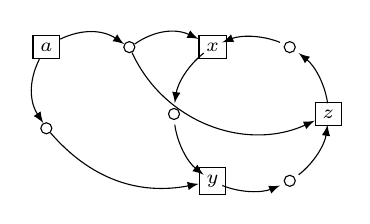
\begin{tikzpicture}[scale=0.7]
\scriptsize
\def \n {6}
\def \radius {1.4cm}
\def \margin {8} % margin in angles, depends on the radius



\node[draw] at ({360/\n * 2}:\radius) (x) {$x$};
\node[draw, circle, minimum size=4pt, inner sep = 0] at ({360/\n * 3}:\radius) {};
\node[draw] at ({360/\n * 4}:\radius) (y) {$y$};
\node[draw, circle, minimum size=4pt, inner sep = 0] at ({360/\n * 5}:\radius) {};
\node[draw] at ({360/\n * 6}:\radius) (z) {$z$};
\node[draw, circle, minimum size=4pt, inner sep = 0] at ({360/\n * 1}:\radius) {};
\foreach \s in {1,...,\n}
{
  
  \draw[->, >=latex] ({360/\n * (\s - 1)+\margin}:\radius) 
    arc ({360/\n * (\s - 1)+\margin}:{360/\n * (\s)-\margin}:\radius);
}

\node[left = 0.8cm of x, draw, circle, minimum size=4pt, inner sep = 0] (sol) {};
\node[left = 0.8cm of sol, draw] (origin) {$a$};
\draw[->, >=latex] (origin) to [bend left] (sol);
\draw[->, >=latex] (sol) to [bend left] (x);
\node[below = 0.8cm of origin, draw, circle, minimum size=4pt, inner sep = 0] (soly2) {};
\draw[->, >=latex] (origin) to [bend right] (soly2);
\draw[->, >=latex] (soly2) to [bend right] (y);
\draw[->, >=latex] (sol) to [bend right= 45] (z);
\end{tikzpicture}
        \caption{$x,y,z$ all have external links, thus none of the links can be discarded}
        \label{cycle3}
    \end{figure}
    
    Cycle $x\to \circ \to y \to \circ \to z\to \circ \to x$ is unbreakable according to Theorem \ref{th:break_cycle}, is possesses 3 incoming edges.
    But with Theorem \ref{th:break_cycle2}, if \textbf{OR gates} are removed, the cycle can be dealt with.
    The removal of \textbf{OR gates} is stated in the next section.
%    If in one cycle, multiple state nodes are required by an external solution node, like in Fig. \ref{cycle3}, cycle $x\to \circ \to y \to \circ \to z\to \circ \to x$ is unbreakable, thus it is a unsolvable case. 
%    From experimental view, this issue never happens to real models to our knowledge but it is an incapability of our approach impeding completeness.
\end{example}

\begin{theorem}\label{th:break_cycle2}
Given a cycle, if it contains no \textbf{OR gate}% towards outside of cycle
, all the local states in the cycles are unreachable.
\end{theorem}

\begin{proof}
Suppose an arbitrary cycle $C=a_i\to \cdots b_j\to\cdots \to a_i$, with $\to$ an edge in the LCG.
Note that $reach'(\alpha,a_i)\implies reach'(\alpha,b_j)\implies reach'(\alpha,b_j.next)\implies \cdots\implies reach'(\alpha,a_i)$.
According to the definition of $reach'$, $reach'(\alpha,a)=\mathbf{True}$ only if $\exists c_k\in C$ and $c_k\in \alpha$.
If there exists such $c_k$, $C$ should not exist as the reasoning stops at $c_k$ and does not form a cycle, contradiction.
$reach'(\alpha,a_i)=reach'(\alpha,b_j)=\cdots =\mathbf{False}$.
\end{proof}
\section{ASPReach Algorithm}
%Our approach is divided into several subroutines. We introduce first the overview then the details of subroutines.
%\subsection{Outline of the Whole Process}\label{sec:outline}
In this section, we present the main contribution of this paper, our analyzer \textbf{ASPReach}: an algorithm for checking the reachability of a target local state $\omega$ from a global initial state $\alpha$ (which can also be partial) in a given ABAN.
However, exhaustive search leads to heavy computation and huge need of memory.
The algorithm proposed below tries to overcome those shortcomings by combining static analysis and stochastic search into the following hybrid approach.


\paragraph{{\bf ASPReach}:}

\begin{itemize}
    \item Input: An ABAN $AB$, an initial state $\alpha$, a target state $\omega$ and a max number of iterations $k$
    \item Output: $reach(\omega)\in\{\mathbf{False},\mathbf{True},\mathbf{Inconclusive}\}$
\end{itemize}
\begin{enumerate}
    \item Construct the LCG $l=LCG(AB,\alpha,\omega)$
    \item Try to remove all cycles and prune useless edges from $l$
    \item Try to prove unreachability of $\omega$ in $l$ using pseudo-reachability $reach'(l,\omega)$ and return $\mathbf{False}$ if $reach'(l,\omega)=\textbf{False}$
    \item Try at most $k$ times
    \begin{itemize}
    \item $l'\gets l$
    %\item  Transform randomly each OR gate $O$ of $l'$ into simple gate
    \item Simplify each \textbf{OR gate} such that $l'$ is a LCG with only \textbf{AND gates}
    \item If there remain cycles:
        \begin{itemize}
            \item Back to step (iv)
        \end{itemize}
    \item Generate all trajectory that starts with $\alpha$ in $l'$ using ASP
    \begin{itemize}
        \item If a trajectory $t$ ending with $\omega$ is found, return $\mathbf{True}$
    \end{itemize}
    \end{itemize}
    \item return $\mathbf{Inconclusive}$
\end{enumerate}

%\subsubsection*{Recap}
%Now all the subroutines are introduced. 
%Among them, only the heuristics at \textbf{OR Gates} is not complete.
LCG illustrates the causality between necessary transitions to be fired to reach the target state; 
the tentative of removing cycles simplifies the LCG and keep the reachability unchanged; 
pseudo-reachability allows one to filter some unreachable cases based on the topology of LCG. 
The heuristic approach is the core of our algorithm.
Stochastic choices avoid combinatorial explosion on different \textbf{OR Gates}.
The ASP part searches thoroughly the result but does not traverse the whole state space (ASP solver starts from constraints, finds one consistent order and terminate the search). 
%It has to be pointed out that INCONCLUSIVE may appear as an output of the Algorithm \ref{algOverall}.
%If the target state $\omega$ is in fact reachable, usually if there exists multiple assignments which contain an admissible solution.
%Moreover, the bigger $k$ we set, the less probable we miss the good assignments.

\begin{algorithm}[htb]
\begin{algorithmic}[1]
\State Input: LCG $l=(V_{\mathrm{state}},V_{\mathrm{solution}}, E)$, an integer $k$
\State Output: reachability $r$ and a trajectory $t$
\State Compute SCCs, classify them into $\mathrm{SCC1}(l)$ with at most 1 incoming edge and $\mathrm{SCC2}(l)$ otherwise
\State \textcolor{gray}{// 1) Break all cycles and prune useless branches}\label{delete_cycle_begin}
\For{each $(V'_{\mathrm{state}} \subseteq V_{\mathrm{state}},V'_{\mathrm{solution}} \subseteq V_{\mathrm{solution}}) \in \mathrm{SCC1}(l)$}
    \For{each $v \in V'_{\mathrm{state}}$}
    \If {$\exists(v,v')\in E, v' \in (V_{\mathrm{solution}} \setminus V'_{\mathrm{solution}})$}
        \State $E\gets E\backslash \{(v,v'')|v''\in V'_{\mathrm{solution}},(v,v'')\in E\}$
    \EndIf
\EndFor
\EndFor \label{delete_cycle_end}
\State{\textcolor{gray}{// 2) remove useless nodes/edges}} \label{prune_begin}
\State pruned = \textbf{True}
\While{pruned}
    \State pruned = \textbf{False}
    \For {$v \in V_{\mathrm{state}}$}
        \If{$\not\exists(v,v')\in E$}
            \State $V_{\mathrm{state}} \gets V_{\mathrm{state}}\backslash \{v\}$; $E\gets E\backslash \{ (v'',v)\in E\}$
            \State $E\gets E\backslash \{ (v'',sol)\in E | sol \in \{sol = (A \rightarrow a) \in V_{\mathrm{solution}} | v \in A\}\}$
            \State $V_{\mathrm{solution}} \gets V_{\mathrm{solution}}\backslash \{sol = (A \rightarrow a) \in V_{\mathrm{solution}} | v \in A\}$
            \State pruned = \textbf{True}
        \EndIf
    \EndFor \label{prune_end}
\EndWhile
\State \textcolor{gray}{// 3) Check pseudo-reachability} \label{pseudo_reach_begin}
\If {$pseudoReach(l)=\textbf{False}$}
    \State \Return $(\mathbf{False},\varnothing)$
\EndIf \label{pseudo_reach_end}

\State \textcolor{gray}{// 4) main search loop} \label{main_loop_begin}
\For{each $i$ in $1\ldots k$}
    \State $l'=(V'_{\mathrm{state}}, V'_{\mathrm{solution}},E')\gets(V_{\mathrm{state}}, V_{\mathrm{solution}},E)$ 
    \For{$v \in V'_{state}$} \textcolor{gray}{// Treat each OR gates}
        \State pick a random element $(v,v') \in E'$
        \State $E'\gets E' \backslash  \{(v,v'') \in E'| v''\neq v'\}$ with $\nexists i\in \mathrm{SCC2}(l)$ and $i\in E'$
    \EndFor
    \State $(r,t)\gets\mathrm{ASPsolve}(l')$
    \If{$r=\textbf{True}$}
        \Return{$(\mathbf{True},t)$}
    \EndIf
\EndFor \label{main_loop_end}
\State \Return{$(\mathbf{Inconclusive},\varnothing)$}
\end{algorithmic}
\caption{ASPReach}\label{algOverall}
\end{algorithm}

Algorithm \ref{algOverall} provides the detailed pseudocode of the algorithm taking an LCG $l$ as input whose detailed construction is given in Algorithm \ref{AlgConstructLCG}.
% Cycle deletion
Lines \ref{delete_cycle_begin}-\ref{delete_cycle_end} delete all cycles with at most one incoming edge.
%Getting rid of cycle prevents self-dependent reachability.
% Pruning
After removing cycles, the LCG may contain nodes without successor.
Such nodes can be pruned since they do not lead to initial state (Line \ref{prune_begin}-\ref{prune_end}).
This preprocessing reduces the search space of the stochastic search performed in step 4.
% Pseudo reach
Now $l$ is pruned and might be cycle-free.
Static analysis of $l$ can then be used as heuristics to check pseudo-reachability (Definition \ref{defPseudoReach}) in order to detect some unreachability cases (Lines \ref{pseudo_reach_begin}-\ref{pseudo_reach_end}) which may conclude before searching.
LCG shows the dependencies between local states and transitions. 
A pathway in LCG suggests a possible trajectory of reaching the target state. 
If $pseudoReach(l,\omega)=\textbf{False}$, we can ensure that $\omega$ is unreachable, as pseudo-reachability checks a necessary condition of reachability.
If $reach'(l,\omega)=\textbf{True}$, static analysis is not sufficient for reachability analysis. 
% St
When static analysis fails, a stochastic search is performed at most $k$ times (line \ref{main_loop_begin}-\ref{main_loop_end}) to find a state sequence from the initial state $\alpha$ to target state $\omega$.
If there remain cycles with multiple incoming edges, according to Theorem \ref{th:break_cycle2}, $\omega$ is unreachable.
The value of $k$ will be discussed later in the evaluation section.
Random choices are made to fix a value for each \textbf{OR gate} of the LCG allowing to perform a reachability check by generating all possible variable assignment order using ASP.
%The detailed of this operation is given in section \ref{sec:OR}.
%After the removal of cycles and the computation of pseudo reachability, the task remains to find a state sequence from the desired state $\omega$ to initial state. 
Keep in mind that every state node is an \textbf{OR gate}, we have to choose one of its successor solution nodes to access the state. 
A set of \textbf{OR gate} choices is called an \textit{assignment}.

\subsection{Stochastic Search}\label{sec:OR}
As every \textbf{OR gate} has multiple choices, to avoid combinatorial explosion, we use a simple heuristic: 
choose randomly one assignment for each trial.
Then we can construct a new LCG without \textbf{OR gate}, every state node has exactly one successor solution node.
%\begin{figure}[ht]
%    \centering
%    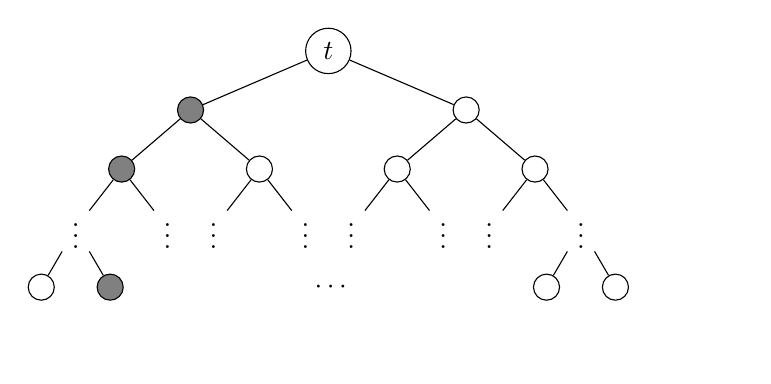
\begin{tikzpicture}[level/.style={sibling distance=70mm/#1},scale=0.5]
\node [circle,draw] (z){$t$}
  child {node [circle,draw,fill=gray] (a) {}
    child {node [circle,draw,fill=gray] (b) {}
      child {node {$\vdots$}
        child {node [circle,draw] (d) {}}
        child {node [circle,draw,fill=gray] (e) {}}
      } 
      child {node {$\vdots$}}
    }
    child {node [circle,draw] (g) {}
      child {node {$\vdots$}}
      child {node (mid) {$\vdots$}}
    }
  }
  child {node [circle,draw] (j) {}
    child {node [circle,draw] (k) {}
      child {node {$\vdots$}}
      child {node {$\vdots$}}
    }
  child {node [circle,draw] (l) {}
    child {node {$\vdots$}}
    child {node (c){$\vdots$}
      child {node [circle,draw] (o) {}}
      child {node [circle,draw] (p) {}
        child [grow=right] {node (q) {} edge from parent[draw=none]
          child [grow=right] {node (q) {} edge from parent[draw=none]
            child [grow=up] {node (r) {} edge from parent[draw=none]
              child [grow=up] {node (s) {} edge from parent[draw=none]
                child [grow=up] {node (t) {} edge from parent[draw=none]
                  child [grow=up] {node (u) {} edge from parent[draw=none]}
                }
              }
            }
            child [grow=down] {node (v) {}edge from parent[draw=none]}
          }
        }
      }
    }
  }
};
\node [right = 2.3cm of e] (point){$\cdots$};
\path (a) -- (j) node [midway] {};
\path (b) -- (g) node [midway] {};
\path (k) -- (l) node [midway] {};
\path (k) -- (g) node [midway] {};
\path (d) -- (e) node [midway] {};
\path (o) -- (p) node [midway] {};
\path (o) -- (e) node (x) [midway] {}
  child [grow=down] {
    node (y) {}
    edge from parent[draw=none]
  };
\path (q) -- (r) node [midway] {};
\path (s) -- (r) node [midway] {};
\path (s) -- (t) node [midway] {};
\path (s) -- (l) node [midway] {};
\path (t) -- (u) node [midway] {};
\path (z) -- (u) node [midway] {};
\path (j) -- (t) node [midway] {};
\path (y) -- (x) node [midway] {};
\path (v) -- (y)
  node (w) [midway] {};
\path (q) -- (v) node [midway] {};
\path (e) -- (x) node [midway] {};
\path (o) -- (x) node [midway] {};
\path (y) -- (w) node [midway] {};
\path (v) -- (w) node [midway] {};
\path (r) -- (c) node [midway] {};
\end{tikzpicture}
%    \caption{Random choice at \textbf{OR gates}, descending from $target$, when we encounter an \textbf{OR gate}, we choose randomly one of its branches. Circles filled gray stand for one possible assignment.}
%    \label{fig:heuristics}
%\end{figure}

After applying heuristics to delete \textbf{OR gates}, we use ASP  (Answer Set Programming) \cite{baral2003knowledge} to analyze the newly obtained LCG with only \textbf{AND gates}.
ASP is a prolog-like declarative programming paradigm.
It uses description and constraints of the problem (called rule) instead of imperative orders.
ASP solver tackles problems by generating all the possibilities respecting the constraints. 
We use Clingo\cite{gebser2016theory} which is a combination of grounder Gringo and solver Clasp. 
Given an input program with first-order variables, grounder computes an equivalent ground (variable-free) program for an ASP program, while solver selects admissible solutions (answer sets) in the ground.

A rule is in the following form:
$$a_0 \gets a_1 , \ldots , a_m, not\ a_{m+1}, \ldots , not\ a_n.$$
where the element on the left of the arrow is called head and the ones on the right called body.
%All the predicates $a_i$, with $0\leq i \leq n$ are replaceable. 
$a_0$ is \textbf{True} if $a_1 , \ldots , a_m$ are \textbf{True} and $a_{m+1}, \ldots , a_n$ are \textbf{False}.
Some special rules are noteworthy. 
A rule where $m = n = 0$ is called a fact and is useful to represent data because the left-hand atom $a_0$ is thus always \textbf{True}.
It is often written without the central arrow.
On the other hand, a rule where $n > 0$ and $a_0 = \perp$ is called a constraint.
As $\perp$ can never become \textbf{True}, if the right-hand side of a constraint is \textbf{True}, this invalidates the whole solution.
Constraints are thus useful to filter out unwanted solutions.
The symbol $\perp$ is usually omitted in a constraint.

Programs can yield no answer set, one answer set, or several answer sets. 
For example, the program \texttt{b:- not c. c:- not b.}  produces two answer sets: $\{b\}$ and $\{c\}$.
Indeed, the absence of $c$ makes $b$ true, and conversely absence of $b$ makes $c$ true. 
Cardinality constraints are another way to obtain multiple answer sets. 
The most usual way of using a cardinality is in place of $a_0$:
$$l \{q_1, \ldots , q_k \} u \gets a_1, \ldots , a_m, not\ a_{m+1}, \ldots , not\ a_n.$$
where $k \geq 0$, $l$ is an integer and $u$ is an integer or $\infty$. 
Such cardinality means that under the condition that the body is satisfied, the answer set $X$ must contain at least $l$ and at most $u$ atoms from the set $\{q_1, \ldots  , q_m\}$, or, in other words: $l \leq |\{q_1, \ldots  , q_m\} \cap X| \leq u$. %where $\cap$ is the symbol of sets intersection and |A| denotes the cardinality of set A.

\subsubsection*{ASP Encoding}

After deleting \textbf{OR gates}, to encode the reachability problem in ASP, we first describe the facts:

Predicate \texttt{init(a,i)} shows the automaton $a$ is at initial state $i$. %\texttt{comp(n,a,i)} shows the joint state $a_i$ needed for transition No.$n$. \texttt{transition(n,b,j)} shows the transition No.$n$ allows the automaton $b$ change to state $j$.
Predicate \texttt{node(a,i,n)} shows the node $a_i$ in the LCG is numbered $n$, while \texttt{parent(n1,n2)} expresses node No.$n_1$ is the predecessor of No.$n_2$.
The LCG in Fig. \ref{fig:limitation} is encoded as follows:
\begin{Verbatim}[commandchars=\\\{\}]
init(a,0). init(b,0). init(c,0).

node(a,1,1). node(b,1,2). node(c,1,3).
node(b,0,4). node(c,0,5).

parent(1,2). parent(1,3).
parent(2,5). parent(3,4).
\end{Verbatim}

After the facts, we want the nodes to appear in an order by which we can fire all the transitions sequentially from initial state to target state. 

The rough idea is: If different states of one automaton $a$ appear, e.g. $a_0$ and $a_1$.
One of them must be in initial state (suppose $a_0$).
The transitions with head $a_0$ have to be fired before $a_0$ flipping to $a_1$, otherwise there is no solution node in the LCG which allows $a_1$ return to $a_0$.
In other words, the predecessor of $a_0$ must appear before $a_1$. \texttt{\textcolor{gray}{Core rule}} describes this constraint.

Predicate \texttt{prior(N1,N2)} signifies node $N_1$ appears earlier than $N_2$ in the resulting state sequence.
\texttt{seq(O,a,i)} shows that state node $a_i$ appears in the O-th place in a trajectory.
\texttt{reachable/unreachable} is the final result of the program.

\begin{Verbatim}[commandchars=\\\{\}]
\textcolor{gray}{%Rule 1, a node appears always earlier than its predecessor}
prior(N1,N2) :- parent(N2,N1).
\textcolor{gray}{%Rule 2, transitivity}
prior(N1,N3) :- prior(N1,N2), prior(N2,N3).
\textcolor{gray}{%Rule 3, Core rule}
prior(N1,N2) :- node(P1,S1,N1), node(P2,S2,N2), node(P2,S3,N3), 
                parent(N1,N3), init(P2,S3), S2!=S3, P1!=P2. 
\textcolor{gray}{%target is unreachable if there is a conflict in order}
unreachable :- prior(N1,N2), prior(N2,N1), N1<N2.
\textcolor{gray}{%One node appears once and at least once in a sequence}
1{seq(1..O,P,S)}1 :- O={node(P1,S1,N1):node(P1,S1,N1)},
                     node(P,S,N), not unreachable.
\textcolor{gray}{%Nodes in the sequence are consistent with the order}
:- prior(N1,N2), node(P1,S1,N1), node(P2,S2,N2),
   seq(O1,P1,S1), seq(O2,P2,S2), O1>O2.
\textcolor{gray}{%One place in the sequence cannot be taken by multiple nodes}
:- seq(O1,P1,S1), seq(O2,P2,S2), P1!=P2, O1=O2.
:- seq(O1,P1,S1), seq(O2,P2,S2), S1!=S2, O1=O2.
\textcolor{gray}{%--------output formatting, displaying initial states first}
:- seq(O1,P1,S1), seq(O2,P2,S2), init(P1,S1),
   not init(P2,S2), O1>O2.
:- seq(O1,P1,S1), seq(O2,P2,S2), init(P1,S1), init(P2,S2),
   P1<P2, O1>O2.
reachable :- not unreachable.
\end{Verbatim}

Notation: $a\rhd b$ means $a$ appears before $b$.

When analyzing the LCG in Fig. \ref{fig:limitation},
Rule 1 gives $b_0\rhd a_1$, $a_1\rhd c_1$, $a_0\rhd b_1$, $b_1\rhd c_1$; Rule 2 gives $a_0\rhd c_1$ and $b_0\rhd c_1$; Rule 3 gives $a_1\rhd b_1$ and $b_1\rhd a_1$ which is impossible, therefore there does not exist a state sequence to reach $c_1$ from initial state.
$c_1$ is unreachable.

If we find a state sequence consistent with all the order constraints, we can obtain its corresponding trajectory, thus we are sure that the target state is reachable.

\begin{figure}[ht]
    \centering
    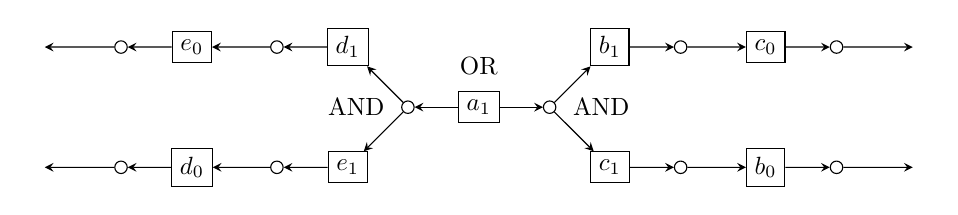
\begin{tikzpicture}[aS,scale=0.9, every node/.style={scale=0.9}]  
  	
  	\startl{a_1};
    \node[Asol,left of=a_1] (a_1s1){};
    \node[Aproc, above left of = a_1s1] (d_1){$d_1$};
    \node[Aproc, below left of = a_1s1] (e_1){$e_1$};
    \node[Asol, left of = d_1](d_1s){};
    \node[Asol, left of = e_1](e_1s){};
    \node[Aproc, left of = e_1s] (d_0){$d_0$};
    \node[Aproc, left of = d_1s] (e_0){$e_0$};
    \node[Asol, left of = d_0](d_0s){};
    \node[Asol, left of = e_0](e_0s){};
    \node[Assol, left of = d_0s](d_0st){$\varnothing$};
    \node[Assol, left of = e_0s](e_0st){$\varnothing$};
    \node[right = 0.1cm of a_1s] {AND};
    \node[left = 0.1cm of a_1s1] {AND};
    \node[above = 0.1cm of a_1] {OR};
    \path 
    (a_1s1) edge (d_1)
    (a_1s1) edge (e_1)
    (d_1) edge (d_1s)
    (e_1) edge (e_1s)
    (d_1s) edge (e_0)
    (e_1s) edge (d_0)
    (d_0) edge (d_0s)
    (e_0) edge (e_0s)
    (d_0s) edge (d_0st)
    (e_0s) edge (e_0st)
    (a_1) edge (a_1s1)
    ; 
  	\specl{above}{a_1}{b_1};
  	\link{b_1}{c_0};
  	\edl{c_0};
  	\specl{below}{a_1}{c_1};
	\link{c_1}{b_0};
  	\edl{b_0};
\end{tikzpicture}

    \caption{If an LCG contains such structure, the result could be inconclusive. However the inconclusiveness requires $a_1$ does not possess other reachable branches. }
    \label{fig:lcgInconc}
\end{figure}
Still, ASPReach is not complete.
A counter-example is shown in Fig. \ref{fig:lcgInconc}, when there are multiple branches of one \textbf{OR gate} leading to unreachability, the result can be inconclusive.
There is a tricky way to deal with this issue when $\mathbf{|OR gates|}$ is not big: we set a limit $n$, if $\mathbf{|OR gates|}<n$, we shift the heuristics on the assignment of \textbf{OR gates} to the enumeration of all possible assignments.
This ``hacking'' can deal with some inconclusiveness.
In the benchmarks in the next section, inconclusive instances appear neither in biological examples nor in random generated tests.

We also show some algorithmic properties of ASPReach:

\begin{theorem}[ASPReach termination and correctness]

    Let $l=(V_{\mathrm{state}}, V_{\mathrm{solution}}, E)$ be an LCG with initial state $\alpha$ and target local state $\omega$ and $k > 0$ be an integer.
    The call \textit{ASPReach(l,k)} terminates.\\
    $ASPReach(l,k)$=$(\mathbf{False},\varnothing)$ only if $\nexists t$ a trajectory in $l$ from $\alpha$ to $\omega$.\\
    $ASPReach(l,k)$=$(\mathbf{True},t)$ only if $\exists t$ a trajectory in $l$ from $\alpha$ to $\omega$.
    The proof is given in appendix \ref{sec:proof}.
\end{theorem}

\begin{theorem}[ASPReach complexity]
    Let $l=(V_{\mathrm{state}}, V_{\mathrm{solution}}, E)$ be an LCG with initial state $\alpha$ and $k > 0$ be an integer.
    Let $s=|V_{\mathrm{solution}}|$ be the number of target state of $l$.
    Let $v = |V_{\mathrm{state}}|$ be the number of vertices of $l$.
    Let $e=|E|$ be the number of edges of $l$.
    The complexity of $\textit{ASPReach(l,k)}$ is $O(v + e + v/2 \times v \times e \times s + v^{2} \times e + v \times e + k \times (v \times e^{2} + 2^{v}))$ which is bound by $O(k \times 2^{v})$.
    Proof is given in Appendix \ref{sec:proof}.
\end{theorem}


\section{Evaluation}
In this section we evaluate our approach through various experiments.
All tests were run on a Intel Core i7-3770 CPU, \@3.4GHz with 8Gb of RAM computer.

To validate our approach, we first tested a small model, $\lambda$-phage model \cite{thieffry1995dynamical} to compare with an alternative reachability analyzer Pint \cite{pauleve2012} implementing solely analysis using LCG \cite{pauleve2017reduction,folschette2015,pauleve2011}.
In this model with 4 automata and 12 transitions (without taking consideration of the self-regulations),
our result shows complete conclusiveness while Pint cannot (Fig. \ref{fig:LCG_lambdaPhage}). %able to figure out the reachability of $cro_1$ when $cl_1$ and $cll_1$ are in the initial state (Fig. \ref{fig:LCG_lambdaPhage}).
PermReach \cite{chai2018heuristic} is not able either to handle some of the special cases where multiple states of one automaton appear in different branches (Fig. \ref{fig:countexPerm}).
Theses cases are solvable by ASPReach.
The whole approach is implemented in Python3\footnote{Code and testing data available at \url{https://github.com/XinweiChai/LCG-in-ASP}}.
The call of ASP is done by package \textit{pyasp}\footnote{\url{https://pypi.python.org/pypi/pyasp}}. 
%In big examples TCR and EGFR, it outputs the sequence from initial state towards final state.
%More importantly, it gives decidable reachability for any input. 

\begin{figure}[ht]
\centering
    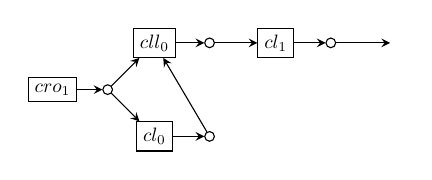
\begin{tikzpicture}[aS,scale=1, every node/.style={scale=0.7}]  
  	
  	\startl{cro_1};
  	\specl{above}{cro_1}{cll_0};
  	\link{cll_0}{cl_1};
  	\edl{cl_1};
  	\specl{below}{cro_1}{cl_0};
	\path (cl_0s) edge (cll_0);
    
    \end{tikzpicture}

    \caption{One LCG in $\lambda$-phage model, automaton $cl$ appears in both branches of the \textbf{AND gate}. Static analyzer Pint cannot decide whether in this case $cro_1$ is reachable or not, because it does not consider the order in the state sequence even though there exists a solution is of length 3: $cll_0::cl_0::cro_1$ corresponding to the trajectory $\acm{cl_1}{cll_1}{cll_0}::\acm{cll_0}{cl_1}{cl_0}::\acm{cll_0,cl_0}{cro_0}{cro_1}$.}
    \label{fig:LCG_lambdaPhage}
\end{figure}
\begin{figure}[ht]
    \centering
    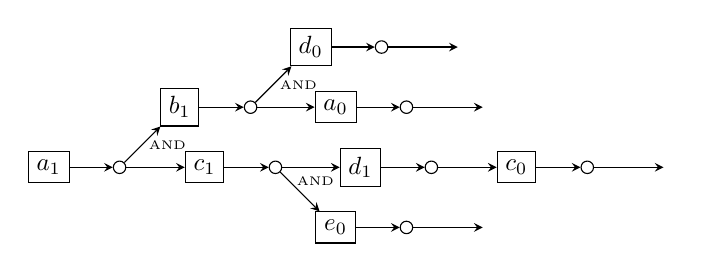
\begin{tikzpicture}[aS, every node/.style={scale=0.9}]  
  	
	\startl{a_1};
	\specl{above}{a_1}{b_1};
	\specl{above}{b_1}{d_0};
	\edl{d_0};
	\link{b_1}{a_0};
 	\edl{a_0};
	\link{a_1}{c_1};
 	\link{c_1}{d_1};
 	\link{d_1}{c_0};
 	\edl{c_0};
 	\specl{below}{c_1}{e_0};
 	\edl{e_0};
 	\node[above right = 0.05cm and 0.2cm of a_1s] {\tiny AND};
 	\node[above right = 0.05cm and 0.2cm of b_1s] {\tiny AND};
 	\node[below right = -0.05cm and 0.1cm of c_1s] {\tiny AND};
    \end{tikzpicture}
    \caption{This counterexample shows former PermReach is inconclusive if multiple states of one automaton appear in the branches of one \textbf{AND gate} ($d_0$ and $d_1$ in this example). 
    However there exists a consistent state sequence: $d_1::b_1::c_1::a_1$ corresponding to the trajectory $\acm{c_0}{d_0}{d_1}::\acm{d_0,a_0}{b_0}{b_1}::\acm{d_1,e_0}{c_0}{c_1}::\acm{b_1,c_1}{a_0}{a_1}$ which could be found by ASPReach.}\label{fig:countexPerm}
\end{figure}

To evaluate the scalability in \textit{in silico} networks, we take T-cell Receptor model (TCR) \cite{saez2007logical} and epidermal growth factor receptor model (EGFR) \cite{samaga2009logic} as examples, with the former one containing 95 automata and 206 transitions and the latter one containing 104 automata and 389 transitions respectively. 

These models are originally Boolean networks.
According to the approach in Appendix \ref{appendix:trans}, BNs are transformed into ABANs. 
Here, we ran the same test as in \cite{folschette2015}. In the TCR model, we take 3 automata as input (\texttt{cd4 cd28 tcrlig}), varying exhaustively their initial states combinations ($2^3$), take the reachability of states of 5 automata (\texttt{sre ap1 nfkb nfat sigmab}) as output. 
Similarly we carried a bigger test on EGFR model with 13 automata %\footnote{\texttt{erbb1 erbb2 erbb3 erbb4 bir btc egf epr nrg1a nrg1b nrg2b nrg4 tgfa}}
as input and 12 automata %\footnote{\texttt{elk1 creb ap1 hsp27 actin\_reorg cmyc pro\_apoptotic p70s6\_2 pkc stat1 stat3 stat5}}
as output.
We first tested the performance of traditional model checkers, Mole\footnote{\url{http://www.lsv.fr/~schwoon/tools/mole}} and NuSMV\footnote{\url{http://nusmv.fbk.eu}}, in which Mole turns out to be memory-out for 6 in 12 outputs, and all memory-out for NuSMV in model EGFR. 
Due to the big state space, traditional model checkers are not applicable.
In the TCR tests, our approach gives exactly the same result as Pint did. 
As for EGFR tests, ASPReach returned no inconclusive output.

\begin{table*}[htb]
    \centering
    \begin{tabular}{|c|c|c|c|c|c|c|}
    \hline
  	Model	&\multicolumn{2}{c|}{$\lambda$-phage}	&	  \multicolumn{2}{c|}{TCR} & \multicolumn{2}{c|}{EGFR}  \\
    \hline
    Inputs&\multicolumn{2}{c|}{4}	&	  \multicolumn{2}{c|}{3} & \multicolumn{2}{c|}{13}\\
    \hline
    Outputs&\multicolumn{2}{c|}{4} &	  \multicolumn{2}{c|}{5} & \multicolumn{2}{c|}{12} \\
    \hline
    Total tests&\multicolumn{2}{c|}{$2^4\times 4=64$} & \multicolumn{2}{c|}{$2^3\times 5=40$} & \multicolumn{2}{c|}{$2^{13}\times 12=98,304$}\\
    \hline
    Analyzer  &  Pint       &\textbf{ASPReach}    &  Pint       &\textbf{ASPReach}   &  Pint       &\textbf{ASPReach}             \\
    \hline
    Reachable    & 36(56\%)& 38(59\%)   &  \multicolumn{2}{c|}{16(40\%)}  & 64,282(65.4\%)&74,268(75.5\%)\\
    \hline
    \textbf{Inconclusive} & \textcolor{red}{\textbf{2(3\%)}}&\textcolor{blue}{\textbf{0(0\%)}}& \multicolumn{2}{c|}{0(0\%)}    &\textcolor{red}{\textbf{9,986(10.1\%)}}&\textcolor{blue}{\textbf{0(0\%)}}  \\
    \hline
    Unreachable     &  \multicolumn{2}{c|}{26(41\%)} &  \multicolumn{2}{c|}{24(60\%)} &24,036(24.5\%)&24,036(24.5\%)\\
    \hline
    Total time &  $<1$s       &  $<1$s &  7s       &  40s        & \textbf{9h50min}              & \textbf{3h46min}      \\
    \hline
    \end{tabular}
    \caption{\label{tab:results}%
    Results of the tests on small ($\lambda$-phage) and large (TCR,EGFR) examples from biology literature. 
    Results of model-checkers using global search are memory-out so are not listed in the table.
    ``Reachable", ``Inconclusive" and ``Unreachable" give respectively the number of different results of reachability.
    It is worth noticing that the inconclusive cases in Pint are caused by time-out \cite{folschette2015}. 
  }
\end{table*}

As seen in Table \ref{tab:results}, our approach can be more conclusive than Pint for ABANs.
In the configuration of heuristics, we set a threshold for \textbf{OR gates}.
If there are less than 10 \textbf{OR gates} after preprocessing, the computation will be shifted from heuristic to the enumeration of all combinations of \textbf{OR gates}.
%It is acceptable for such a model, i.e. at most $2^{10}$ paths to check. 
Here is the case for these three benchmarks. The experiments show the ability of ASPReach is already more conclusive than Pint in ``simple'' cases.

%In addition, when running these tests, we noted the maximum (6) and the average (1.006) of iterations $k$. 


%\begin{table*}[htb]
%    \centering
%    \begin{tabular}{|c|c|c|c|c|}
%        \hline
%        Analyzer & Exhaustive ASPReach & ASPReach& PermReach&Pint\\
%        \hline
%        Inconclusive & 0&52&61&123\\
%        \hline
%    \end{tabular}
%    \caption{\label{tab:compPermReach}Result of 16000 random tests. Exhaustive ASPReach runs a search on every possible assignment on OR gates thus is firmly conclusive. ASPReach, PermReach and Pint result in inconclusive cases. Except inconclusive cases, the results are consistent between different approaches.}
%\end{table*}

To test the global applicability of ASPReach, we ran two sets of tests on random models generated as follows: 
Given the number of transitions, for every transition $tr$, the head $a_h$ is randomly chosen from $LS$, the first element of the body $A_1$ is chosen from $LS_1=LS\setminus \{a_h,a_{1-h}\}$.
For $i>1$, if $A_{i-1}=b_x$ exists, we generate $A_i$ with an 80\% probability, choosing from $LS_i=LS_{i-1}\setminus \{b_x,b_{1-x}\}$. 

Fig. \ref{fig:sizeTest} shows the average run time of ASPReach on randomly generated ABAN.
In this experiment, we fixed the number of transitions to $|\Sigma|\times 3$ and each transition has a random number of heads from 1 to $|\Sigma-1|$, with $\Sigma$ the number of automata of the generated ABAN.
For traditional model checkers like NuSMV and Mole, memory-out cases begin to appear when $|\Sigma|>50$, so the runtime results are not displayable in Fig. \ref{fig:sizeTest}. 
Also, Pint is not able to check all test sets of any $|\Sigma|$.
Even though the curve of average runtime of our approach shows an exponential-like tendency, ASPReach is very fast for $|\Sigma|<100$ (less than 0.03s) and can also perform on models with 1000 automata.
Moreover, the longest runtime among the test sets is less than 20s. 
Because we stop the computation if one reachability check takes more than 20s and we note it as timeout.
This result suggests that the heuristic approach of ASPReach has a good performance in conclusiveness in general as the testing models are generated randomly.

Another test is on the different density with the same number of automata. 
In Fig. \ref{fig:inconcTest}, we fixed $|\Sigma|=20$ and vary the number of the transitions per automaton (density) from 1 to 12.
The runtime peak is at density 8, a possible explanation is that even the topology of the network is more complex with the growth of density, more available transitions lead to more pathways from the initial state to the target state, thus the heuristics may end with less trials.

\begin{figure}[ht]
    \subfigure[0.5\textwidth][ABAN density fixed to 3]{
    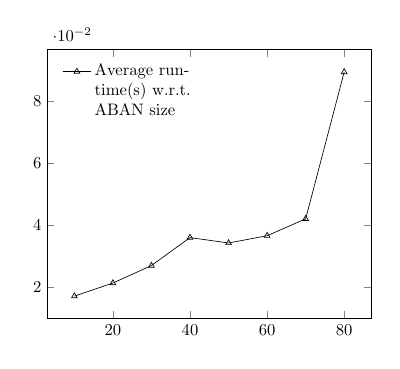
\begin{tikzpicture}[>=stealth,scale=0.6,line width=0.8pt]
    \begin{axis}%[legend pos=north west]
       \addplot[mark=triangle] coordinates{
        (10,6.8/8*0.02)
        (20,8.5/8*0.02)
        (30,10.76/8*0.02)
        (40,14.38/8*0.02)
        (50,13.68/8*0.02)
        (60,14.62/8*0.02)
        (70,16.8/8*0.02)
        (80,35.8/8*0.02)
        };
        \addlegendentry{Average runtime(s) w.r.t. ABAN size}
    \end{axis}
\end{tikzpicture}

    \label{fig:sizeTest}
    }
    \subfigure[0.5\textwidth][ABAN size fixed to 20]{
        \centering
    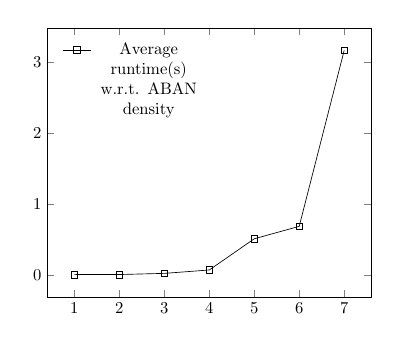
\begin{tikzpicture}[>=stealth,scale=0.6,line width=0.8pt,align=center]
    \begin{axis}%[legend pos=north west]
       \addplot[mark=square] coordinates{
        (1,3.57/400)
        (2,3.9/400)
        (3,10.4/400)
        (4,29.4/400)
        (5,205/400)
        (6,275/400)
        (7,1265/400)
        };
        \addlegendentry{Average runtime(s) w.r.t. ABAN density}
    \end{axis}
\end{tikzpicture}

    \label{fig:inconcTest}
    }
    \caption{Runtime of ASPReach on random ABANs}
\end{figure}


These experimental evaluations show that ASPReach has a better scalability on reachabilty analysis than traditional exhaustive model checkers and a better performance regarding conclusiveness than existing static analyzer.


\section{Conclusion}
In this paper, we present the ABAN modeling framework and its model-related reachability analyzer ASPReach.
%ABAN subsumes asynchronous Boolean network and is more expressive than the latter as its transitions can be asymmetric.
Facing the two critical challenges: complexity and conclusiveness, we combine static analysis and Answer Set Programming for a good performance on both criteria.
ASPReach performs normally on models with $1000$ automata while traditional model checkers fail to compute and static analyzer Pint also fails to give conclusive results on certain instances.

We are now considering an incorporation of heuristics in the preprocessing phase, like the work of \cite{PRNs-TCS18}, to improve the performance of our approach regarding runtime.
The development of dedicated heuristic for the orientation of the random search in ASPReach remains also a future work.

As to biological application, one path of research is the interfacing of our approach with model inference approaches.
Biological models can be inferred from experimental data through machine learning techniques (e.g. \cite{inoue2014learning}), but obtained models are not necessarily consistent with the \textit{a priori} background knowledge about the dynamics of system. 
Thus it is important to check these obtained models and revise them to make them consistent with such background knowledge.
In the case of reachability properties, our approach could be use as a model checker and a mean to enforce such properties in a model under construction.

\bibliographystyle{plain}
\bibliography{bib}

\appendix

\section{Transformation from BNs to ABANs}\label{appendix:trans}

Given Boolean functions $v_i(t+1)=f_i(\mathbf{V}_i)$, with $\mathbf{V}_i$ the set of participating variables among $v_1(t),\cdots,v_n(t)$.
Boolean functions could be transformed to equivalent CNF (conjunctive normal form) and DNF (disjunctive normal form) if the length of Boolean functions is limited to $O(1)$ \cite{miltersen2005converting} which is often the case.
\begin{proposition}[Transformation from BN to ABAN]
Given a BN $G_B=(V,F)$, with its functions in CNF form $v^i(t+1)=A_1\land\ldots A_j \ldots\land A_n$ and DNF form $v^i(t+1)=A'_1\lor\ldots A_k\ldots\lor A'_m$, an equivalent ABAN $AB$ has transitions $A_j\to v^i_1$ and $\lnot A_k\to v^i_0$ where $A_j$ are disjunctions and $A'_K$ are conjunctions.
\end{proposition}
\begin{example}
Let $G_B=(V,F)$ a BN with $V=\{a,b,c,d,e\}$, and has only one Boolean function, $F=\{f(a)= (b\lor c)\land(d\lor e)\}$, we have 
$f(a)=(b\land d)\lor(b\land e)\lor(c\land d)\lor(c\land e)$, and $\lnot f(a)=(\lnot b\land \lnot c)\lor(\lnot d\land \lnot e)$. 
The equivalent ABAN is then constructed: 5 automata $\mathbf{\Sigma}=\{a,b,c,d,e\}$, with transitions: $\mathbf{T}=\{\acm{b_1,d_1}{a_0}{a_1},\ \acm{b_1,e_1}{a_0}{a_1},\ \acm{c_1,d_1}{a_0}{a_1},\ \acm{c_1,e_1}{a_0}{a_1},\ \acm{b_0,c_0}{a_1}{a_0},\ \acm{d_0,e_0}{a_1}{a_0}\}$.
\end{example}

\section{Proofs}\label{sec:proof} %of Theorem of section \ref{sec:ASP}}

\begin{theorem}[ASPReach termination and correctness]
    
    Let $l=(V_{\mathrm{state}}, V_{\mathrm{solution}}, E)$ be an LCG with initial state $\alpha$ and target local state $\omega$ and $k > 0$ be an integer.
    The call \textit{ASPReach(l,k)} terminates.\\
    $ASPReach(l,k)$=$(\mathbf{False},\varnothing)$ only if $\nexists t$ a trajectory in $l$ from $\alpha$ to $\omega$.\\
    $ASPReach(l,k)$=$(\mathbf{True},t)$ only if $\exists t$ a trajectory in $l$ from $\alpha$ to $\omega$.
    \begin{proof}
    
        1: The algorithm starts by breaking all cycles of the LCG and according to Theorem \ref{th:break_cycle} it terminates and does not affect the reachability of $\alpha$ in $l$.
        
        2: Then all nodes of $V_{\mathrm{state}}$ and (resp. ${\mathrm{solution}}$) with no (resp. missing) outgoing edges are removed.
        Such nodes cannot be part of a trajectory leading to initial state $\alpha$ and thus this operation does not affect the reachability of $\alpha$ in $l$.
        The internal for loop of this operation iterates over $V_{\mathrm{state}}$ which is finite.
        To continue looping, it requires one state deletion thus this operation will terminate atleast when $V_{\mathrm{state}}$ becomes $\varnothing$.
        
        Conclusion 1: $ASPReach(l,k)=\mathbf{False}$ only if $\nexists t$ a trajectory in $l$ from $\alpha$ to $v \in V_{\mathrm{solution}}$.
        
        Conclusion 2: the call \textit{ASPReach(l,k)} terminates.
        
        Conclusion 3: After this pre-processing, pseudo reachability is checked and according to \cite{pauleve2012}, it terminates and is correct.
        It is the only possibility for ASPReach to output $\mathbf{False}$.
        
        Conclusion 4: Stochastic search follows by randomly reducing each OR gate of $l$ to one of its edges to form $l'$.
        This operation is run a finite time $k$ and iterates over $V_{\mathrm{state}}$ which is finite and thus it terminates.
        This operation does not create new edges, i.e. $E' \subseteq E$.
        $ASPsolve(l')$ generates all possible trajectories of $l'$ leading to $\alpha$.
        The number of possible trajectory is finite and thus $ASPsolve(l')$ terminates.
        
        
        
        Furthermore when $ASPsolve(l')=(\mathbf{True},t)$, t is a trajectory of $l$ proving reachability of $\alpha$ in $l$ and it is the only possibility for ASPReach to output $\mathbf{True}$.
        
        Conclusion 3: $ASPReach(l,k)=(\mathrm{\mathbf{True}},t)$ only if $\exists t$ a trajectory in $l$ from $\alpha$ to $v \in V_{\mathrm{solution}}$.
    \end{proof}
\end{theorem}

\begin{theorem}[ASPReach complexity]
    Let $l=(V_{\mathrm{state}},V_{\mathrm{solution}}, E)$ be an LCG with initial state $\alpha$ and $k > 0$ be an integer.
    Let $s=|V_{\mathrm{solution}}|$ be the number of target state of $l$.
    Let $v = |V_{\mathrm{state}}|$ be the number of vertices of $l$.
    Let $e=|E|$ be the number of edges of $l$.
    The complexity of $ASPReach(l,k)$ is $O(v + s + e + (v+s) / 2 \times v \times e \times s + v^{2} \times e + v \times e + k \times (v \times e^{2} + 2^{v}))$ which is bound by $O(k \times 2^{v})$.
    \begin{proof}
    
        1: computing $SCC(l)$ has a complexity of $O(v + s + e)$.
        In worst case $|SCC(l)| = (v+s) / 2$ and breaking one cycle of $SCC(l)$ is $O(v \times e \times s)$, thus complexity of removing cycle is $op1=O(v+ e + s + (v+s) / 2 \times v \times e \times s)$
        
        2: To remove useless nodes ASPReach iterates over all states and checking if one state has no successor in $l$ requires to iterates over all edges.
        In worst case all states will be removed one by one and thus the complexity of this operation is $op2=O(v \times (v+s) \times e)$.
        
        3: Computing pseudo reachability over $l$ which have no loop correspond to perform a depth first search on all branch of a tree and thus bound to $op3=O((v+s) \times e)$.
        
        4: the stochastic search iterates atmost $k$ times.
        Treating each OR gate to form $l'$ have a cost of $O(v \times e \times e)$
        $ASPsolve(l')$ generates trajectories that can prove reachability of $\alpha$ in $l'$.
        Each trajectory is a sequence where each element of $|V_{\mathrm{state}}|$ appears exactly once.
        It correspond to the number of total order of $|V_{\mathrm{state}}|$ which is $2^{v}$.
        % TODO: the asp program never produce two times the same sequence ?
        Thus $ASPsolve(l')$ is bound by $O(2^{v})$ and the whole stochastic search by $op4=O(k \times (v \times e^{2} + 2^{v}))$.
        
        Conclusion 1: The complexity of $ASPReach(l,k)$ is $O(op1 + op2 + op3 + op4) = O(v + e + s + (v+s) / 2  \times v \times e \times s + v \times (v+s) \times e + v \times e + k \times (v \times e^{2} + 2^{v}))$.
        
        Conclusion 2: The complexity of $ASPReach(l,k)$ is bounded by $O(k \times 2^{v})$
    \end{proof}
\end{theorem}

\section{Pseudo Code of Pseudo-reachability}

\begin{algorithm}[ht]
\begin{algorithmic}
\State Input: an LCG $l=(V_{\mathrm{state}}, {V_\mathrm{solution}},E)$, an initial state $\alpha$, a target state $\omega$
\State Output: a Boolean $reach'$
\Procedure{pseudoReach}{$s$}
\State \textcolor{gray}{// If $\omega$ is in initial state, it is already reached}
\If {$\omega\in \alpha$}
   \Return \textbf{True}
\EndIf
%\State \textcolor{gray}{// If no solution nodes leads to $s$, $s$ is unreachable}
\State \textcolor{gray}{// The reachability of $s$ depends on its successor solution nodes}
\If {$\not\exists (s,sol) \in E$}
    \Return \textbf{False}
\EndIf
\For{each $(s,sol) \in E$}
    \If{\Call{fireable}{$sol$}}
    \Return \textbf{True}
    \EndIf
\EndFor
 \Return \textbf{False}
\EndProcedure
\Procedure{fireable}{$sol$}
\For{each $(sol,s') \in E$}
    \If{\Call{pseudoReach}{$s'$}}
    \Return \textbf{False}
    \EndIf
\EndFor
\Return \textbf{True}
\EndProcedure
\end{algorithmic}
\caption{Pseudo-reachability $reach'$}\label{algPseudo}
\end{algorithm}
\end{document}
